	


\newpage
%-----------------------------------------------------------------------------
\section{} 
	\textbf{Гомотопия отображений. Согласованность гомотопии с композициями. Гомотопия относительно подмножества. Пример: линейная гомотопия отображений со значениями в выпуклом подмножестве $\mathbb{R}^n$}\\
	\\
	\begin{figure}[h]
		\center{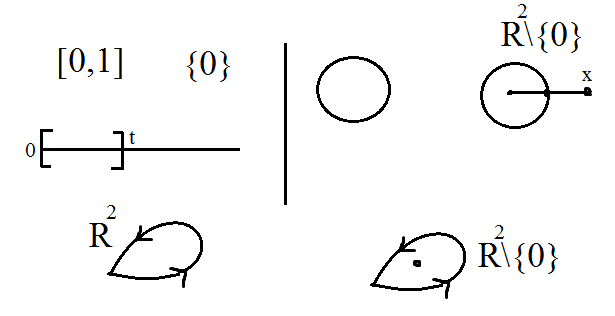
\includegraphics[scale = 0.6]{1-1.png}}
	\end{figure}\\
	\textbf{Обозначение}: $I = [0,1]$\\
	\textbf{Определение}: $X,Y$ -- топологические пространства, $f,g:\ X \rightarrow Y$ -- непрерывны. Гомотопия между $f$ и $g$ -- непрерывное $F:\ X \times I \rightarrow Y$, такое что $F(x,0) = f(x),\ F(x,1) = g(x) \forall x\in X$\\
	\textbf{Замечание}: $F$ порождает семейство $\{F_t:\ X \rightarrow Y\} t\in U,\ F_t(x) = F(x,t)\\
	F_0 = f,\ F_1 = g$\\
	\textbf{Обозначение}: $F:\ f \simeq g$\\
	\textbf{Определение}: $f$ и $g$ гомотопны $\Leftrightarrow$ существует гомотопия $F:\ f \simeq g$\\
	\textbf{Предложение}: $\simeq$ -- отношение эквивалентности на $C(X,Y)$\\
	\textbf{Лемма(о склейке)}:\\
	$X,Y$ -- топологические пространства, $f:\ X\leftarrow Y,\ X = \underset{i\in I}{\cup} X_i, {f|}_{X_i}$ непрерывно $\forall i$\\
	Предположим, что выполнено одно из следующих условий:
	\begin{enumerate}
		\item все $X_i$ открыты
		\item все $X_i$ замкнуты и $I$ конечно
	\end{enumerate}
	Тогда $f$ непрерывно\\
	\textbf{Доказательство}:\\
	\begin{enumerate}
		\item очевидно
		\item для любого замкнутого $B\subset Y f^{-1} (B) = \underset{i\in I}{\cup} (f^{-1}(B) \cap X_i) = \underset{i\in I}{\cup} {f_i}^{-1} (B),\ \text{где} f_i = {f|}_{X_i}\\
		f^{-1} (B)$ замкнуто в $X_i$, то есть $f_i$ -- непрерывно $\Rightarrow {f_i}^{-1} (B)$ замкнуто в $X \Rightarrow f^{-1} (B)$ замкнуто и $f$ непрерывно
	\end{enumerate}
	\textbf{Доказательство предложения}:\\
	\begin{enumerate}
		\item $f\simeq f$: положим $F(x,t) = f(x) \forall x, \forall t$
		\item Пусть $F: f \simeq g, G: g\simeq h$. Положим, $G(x,t) = F(x, 1-t) \forall x, \forall t \Rightarrow G: g \simeq f$
		\item Пусть $F: f\simeq g, G: g\simeq h$. Положим $H(x,t) = 
		\begin{cases}
			F(x, 2t)\ if\ 0 \leq t \leq \frac{1}{2}\\
			G(x, 2t-1)\ if\ \frac{1}{2} \leq t \leq 1
		\end{cases}$
		$\Rightarrow H: f \simeq g$. Непрерывность $H$ -- из леммы о склейке
	\end{enumerate}
	\begin{figure}[h]
		\center{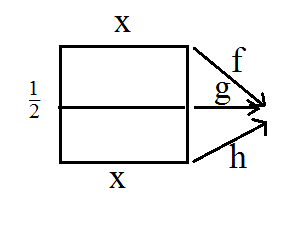
\includegraphics[scale = 0.6]{1-2.png}}
	\end{figure}
	\textbf{Предложение}: $f_0, f_1:\ X \rightarrow Y,\quad g_0, g_1:\ Y \rightarrow Z,\ f_0 \simeq f_1,\ g_0 \simeq g_1\ \Rightarrow\ g_0 \circ f_0 \simeq g_1 \circ f_1$\\
	\textbf{Доказательство}: пусть $F:\ f_0 \simeq f_1,\quad G:\ g_0 \simeq g_1$\\
	Рассмотрим $H:\ X \times I\ \rightarrow Z,\ H_t\slash G_t \circ F_t \forall t\in I,\ \text{то есть}\ H(x,t) = G(F(x,t),t)\ (x\in X, t\in I)$\\
	$H$ -- непрерывно, $H: g_0 \circ f_0 \simeq g_1 \circ f_1$ что и требовалось доказать\\
	\textbf{Определение}: $X, Y$ -- топологические пространства, $A\subset X, f,g:\ X\rightarrow Y$ непрерывно, ${f|}_A = {g|}_A$\\
	Гомотопия $F: f\simeq g$ называется гомотопией относительно $A (A$-гомотопией) $\Leftrightarrow {F_t |}_A = {f|}_A \forall t\in I$\\
	Обозн: $F: f \underset{A}{\simeq} g$\\
	\textbf{Определение}: $f$ и $g A$ -- гомотопии ($f \underset{A}{\simeq} g) \Leftrightarrow \exists F: f\simeq g$\\
	\textbf{Предложение}: (1) $\forall \phi \in C(A,Y)$ отношение $\underset{A}{\simeq}$ является отношением эквивалентности на $\{ f\in C(X,Y): {f|}_A = \phi \}$\\
	(2)$f_0, f_1: X\rightarrow Y, g_0 \circ g_1: Y\rightarrow Z$ непрерывно, $f_0 \underset{A}{\simeq} f_1, g_0 \underset{B}{\simeq} g_1 (где f_0 (A) \subset B) \Rightarrow g_0 \circ f_0 \underset{A}{\simeq} g_1 \circ f_1$\\
	\textbf{Доказательство}: аналогично случаю $A = B = \varnothing$ (см.выше)\\
	Примечание: $X$ -- топологические пространство, $Y$ -- нормированное пространство, $z\subset Y$ выпуклое\\
	Покажем: $\forall A\subset X$ любые непрерывные $f,g: X\rightarrow Z$, такие, что ${f|}_A = {g|}_A, f$ и $g A$-гомотопии\\
	В частности: любые два непрерывных $X\rightarrow Z$ гомотопии\\
	Рассмотрим $F: X\times I \rightarrow Z, F(x,t) = tg(x) + (1-t) f(x)$ (линейная гомотопия)\\
	\begin{figure}[h]
		\center{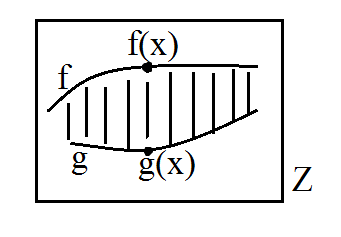
\includegraphics[scale = 0.6]{1-3.png}}
	\end{figure}\\
	


\newpage
%-----------------------------------------------------------------------------
%2 done 
	\section{} 
	\textbf{Гомотопия путей. Пример: замена параметра. Прозведение путей и их гомотопический классов. Свойства операции умножения гомотопических классов путей. Фундаментальная группа.}\\
	\\
	$X$ -- топологические пространство, $x_0, x_1 \in X$\\
	\textbf{Определение}: Путь в $X$ из $x_0$ в $x_1$ -- непрерывен и $I\rightarrow X,\ u(0) = x_0,\ u(1) = x_1$\\
	Петля в $x_0$ -- путь из $x_0$ в $x_0$\\
	$P(x_0, x_1) = \{ \text{пути в}\ X\ \text{из}\ x_0\ \text{в}\ x_1\}$\\
	\textbf{Определение}: $u, v \in P(x_0, x_1)$ гомотопны, как пути $\Leftrightarrow u\simeq v \Leftrightarrow \exists$ гомотопия $F:\ u\simeq v$, такие что $\forall t\in I,\ F_t \in P(x_0,x_1)$, то есть $F(0,t) = x_0,\ F(1,t) = x_1,\ \forall t$\\
	\textbf{Обозначение}: $u \underset{p}{\simeq} v$\\
	\textbf{Обозначение}: $\Pi (x_0, x_1) = P(x_0, x_1)\diagup \underset{p}{\simeq}$ -- множество гомотопических классов путей из $x_0$ в $x_1$, $\forall u\in P(x_0,x_1)$ Обознаяение $[u]$ -- его гомотопический класс в $\Pi(x_0,x_1)$\\
	\textbf{Обозначение}: $\pi_1 (X,x_0) = \Pi(x_0, x_1)$ -- множество гомотопических классов петель в $x_0$\\
	\textbf{Определение}: пусть $u\in P(x_0,x_1),\ v\in P(x_1,x_2)$\\
	Произведение $u,v$ -- путь $uv \in P(x_0,x_2), (uv)(S) = 
	\begin{cases}
	u(2S)\ if\ S \leq \frac{1}{2}\\
	v(2S-1)\ if\ S \geq \frac{1}{2}
	\end{cases}$\\
	\textbf{Замечание}: то, что выше обозначается $uv$, иногда обозначается $vu$\\
	\textbf{Предложение}: $u_0, u_1 \in P(x_0,x_1),\ v_0,v_1 \in P(x_1,x_2) u_0 \underset{p}{\simeq}\ u_1, v_0 \underset{p}{\simeq} v_1 \Rightarrow u_0 v_0 \underset{p}{\simeq} u_1 v_1$\\
	\textbf{Доказательство}: пусть $F: u_0 \underset{p}{\simeq} u_1,\ G: v_0 \underset{p}{\simeq} v_1$\\
	Рассмотрим $H: I\times I\ \rightarrow\ X, H_t = F_t \cdot G_t,\ \forall t\in I$, то есть $H(S,t) = 
	\begin{cases}
	F(2S, t)\ if\ S \leq \frac{1}{2}\\
	G(2S-1,t)\ if\ S \geq \frac{1}{2}
	\end{cases}$\\
	$H$ непрерывно (по лемме о склейке), $H: u_o v_o \underset{p}{\simeq} u_1 v_1$
	Следствие: определено отображение:\\
	$\Pi (x_0,x_1) \times \Pi (x_1, x_2) \rightarrow \Pi(x_0, x_2)\\
	([u], [v]) \rightarrow [u][v] = [uv]$ (опр)\\
	Обозн: (1) $\forall x_0 \in X, e_{x_0}: I \rightarrow X, e_{x_0} (S) = x_0, \forall S\in I\\
	(2)\forall u\in P(x_0,x_1) u^{-1} \in P(x_1,x_0), u^{-1} (S) = u(1-S)\ \forall S\in I$
	Лемма(о замене параметра)\\
	Пусть $\phi: I \rightarrow I$ непрерывно, $\phi(0) = 0, \phi(1) = 1 \Rightarrow \forall u \in P(x_o,x_1)$\\
	\textbf{Доказательство}: $I$ выпукло $\Rightarrow\ \phi \underset{\{0,1\}}{\simeq}  \text{id}_I\ \Rightarrow\ u\cdot \phi \underset{\{0,1\}}{\simeq} u$\\
	\begin{figure}[h]
		\center{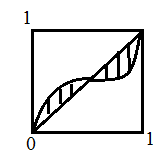
\includegraphics[scale = 0.6]{2-1.png}}
	\end{figure}\\
	\textbf{Теорема}: 
	\begin{enumerate}
		\item $[e_{x_e}][u] = [u] = [u][e_{x_1}]\ \forall u\in P(x_0,x_1)$
		\item $[u][u^{-1}] = [e_{x_0}], [u^{-1}][u] = [e_{x_1}]\ \forall u\in P(x_0,x_1)$
		\item $([u][v])[w] = [u]([v][w])\ u\in P(x_0,x_1),\ v\in P(x_1,x_2),\ w\in P(x_2,x_3)$
	\end{enumerate}
	\textbf{Доказательство}: 
	\begin{enumerate}
		\item 
		\begin{figure}[h]
			\center{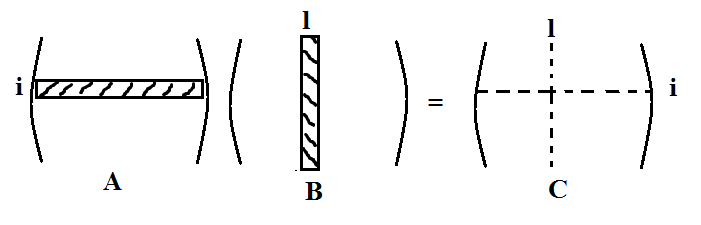
\includegraphics[scale = 0.6]{2-2.png}}
		\end{figure}
		Рассмотрим $\phi: I\rightarrow I$ (см.рис)\\
		$u\cdot \phi = e_{x_0} u \Rightarrow u \underset{p}{\simeq} e_{x_0} u$\\
		Аналогично $u \simeq u\cdot e_{x_1}$
		\item 
		\begin{figure}[h]
			\center{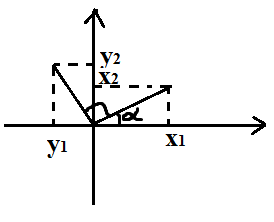
\includegraphics[scale = 0.6]{2-3.png}}
		\end{figure}
		Рассмотрим $F: I\times I \Rightarrow X$\\
		\begin{gather*}
		F(S,t) = 
		\begin{cases}
		u(2S)\ if\ S \leq \frac{t}{2}\\
		u(t)\ if\ \frac{t}{2} \leq S \leq 1 - \frac{t}{2}\\
		v(2S-1)\ if\ 1 - \frac{t}{2} \leq s \leq 1
		\end{cases}
		\end{gather*}
		$F: e_{x_0} \simeq uu^{-1}$, непрерывность $F$ - из леммы о склейке\\
		меняем ролями $u,u^{-1} \Rightarrow$ получаем $e_{x_1} \simeq u^{-1}u$
		\item 
		\begin{figure}[h]
			\center{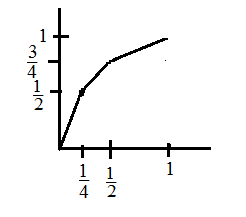
\includegraphics[scale = 0.6]{2-4.png}}
		\end{figure}
		Рассмотрим $\phi: I\Rightarrow I$ (см.рис)\\
		$(u\cdot (v\cdot w))\cdot \phi = (u\cdot v)\cdot w \Rightarrow u\cdot (v\cdot w) \underset{p}{\simeq} (u\cdot v)\cdot w$ что и требовалось доказать
	\end{enumerate}
	\textbf{Следствие}: операция произведения гомотопных кассов петель превращает ${\pi}_1 (X,x_0)$ в группу. Её нейтральный элемент $[e_{x_0}],\ [u]^{-1} = [u^{-1}]\ \forall u \in {\pi}_1 (X, x_0)$\\
	\textbf{Определение}: ${\pi}_1 (X,x_0) $ -- фундаменталная группа $X$ в $x_0$\\
	\textbf{Пример}: Если $Z$ выпуклое подмножество нормированного пространства $X$, то $\forall x_0 \in Z\ {\pi}_1 (Z,x_0)$ -- тривиальна
	
	


\newpage
%-----------------------------------------------------------------------------
%4 done 
	\section{}
	\textbf{Поднятия отображений $Y \rightarrow S^1$ до отображений $Y \rightarrow \mathbb{R}$: единственность (для произвольного связного пространства $Y$) и существование (для компактного звездного помножества $Y\subset \mathbb{R}^n$)}\\
	
	Определение: $Y$ -- топологические пространство, $f: Y \rightarrow S^1$ непрерывно. Непрерывное оторбражение $g: Y \rightarrow \mathbb{R}$ называется поднятием $f \Leftrightarrow pog = f$\\
	\begin{figure}[h]
		\center{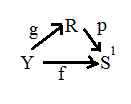
\includegraphics[scale = 0.6]{4-1.png}}
	\end{figure}\\
	Предложение (о единственности поднятия): $Y$ -- связное топологическое пространство, $f: Y \rightarrow S^1$ непрерывно, $g_1, g_2: Y \rightarrow \mathbb{R}$ -- поднятия $f$\\
	Предположим: $\exists y_0 \in Y, такое что g_1(y_0) = g_2(y_0) \Rightarrow g_1 = g_2$\\
	\textbf{Доказательство}: рассмотрим $g: Y \rightarrow \mathbb{R}, g = g_1 - g_2, g$ непрерывно\\
	$pog_1 = pog_2 \Rightarrow \forall y \in Y p(g(y)) = \frac{p(g_1 (y))}{p(g_2 (y))} = 1 \Rightarrow g(Y) \subset \mathbb{Z}, g(Y)$ связно\\
	$0 = g(y_0) \in g(Y) \Rightarrow g(Y) = \{0\} \Rightarrow g_1 = g_2$ что и требовалось доказать\\
	\textbf{Определение}: $X$ векторное пространство над $\mathbb{R}, Y\subset X, y_0 \in Y$\\
	$Y$ -- звездное относительно $y_0 \Rightarrow \forall y\in Y$ отрезок $[y_0, y] \subset Y$\\
	Предложение (о существовании поднятия): Пусть $X$ -- нормированное пространство над $\mathbb{R}, Y\subset X$ -- компактное множество, звездное относительно $y_o \in Y$\\
	Тогда для любого непрерывного $f: Y\rightarrow S^1, \forall t_0 \in \mathbb{R}$, такое что $p(t_0) = f(y_0)$, существует непрерывное $g: Y\rightarrow \mathbb{R}$, поднимающее $f$ и такое что $g(y_0) = t_0$\\
	\textbf{Доказательство}: Можем считать, что $y_0 = 0$\\
	Из равномерной непрерывности $f: \exists \delta \textgreater 0$, такое что $\forall y, y^{\prime} \in Y$, удовлетворяющие $||y-y^{\prime}|| \textless \delta$, выполнено $|f(y)-f(y^{\prime})| \textless 2$ (то есть $f(y) \neq -f(y^{\prime})$) Обозначим $C = sup \{||y||: y\in Y\}, C \textless \infty$, так как $Y$ -- ограничено\\
	Зафиксируем $n\in \mathbb{N}$, такое что $\frac{C}{n} \textless \delta$\\
	\begin{figure}[h]
		\center{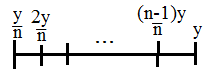
\includegraphics[scale = 0.6]{4-2.png}}
	\end{figure}\\
	$\forall k = 0, \ldots , n-1\quad \forall y\in Y\quad || \frac{(k+1)y}{n} - \frac{ky}{n}|| = \frac{||y||}{n} \textless \delta \Rightarrow f(\frac{(k+1)y}{n})\slash f(\frac{ky}{n}) \neq -1$\\
	Обозначим $f_k:\ Y \rightarrow S^1 \diagup \{-1\},\quad f_k (y) = f(\frac{(k+1)y}{n})\slash f(\frac{ky}{n}),\quad f_k$ -- непрерывно\\
	Заметим: $f(y) = f(0) f_0 (y) f_1 (y) \ldots  f_{n-1} (y)\quad \forall y\in Y$\\
	Рассмотрим $g:\ Y\rightarrow \mathbb{R}, g(y) = t_0 + S(f_0 (y)) + S(f_{n-1} (y)), g$ непрерывно, $p \circ g = f,\ g(0) = t_0$ что и требовалось доказать



\newpage
%-----------------------------------------------------------------------------
%5 done
	\section{} 
	\textbf{Степень( = вращение) петли $[0,1] \rightarrow (S^1, 1)$. Свойства степени. Фундаментальная группа окружности.}\\
	Фундаментальная группа окружности.\\
	\\
	\textbf{Обозначение}: $S^1 = \{ z\in \mathbb{C}: |z| = 1\}\\\
	p: \mathbb{R} \rightarrow S^1, p(t) = e^{2\pi it}$\\
	\textbf{Предложение}: ${p|}_{(- \frac{1}{2}, \frac{1}{2})}$ -- гомеоморфно $(- \frac{1}{2}, \frac{1}{2})$ на $S^1 \diagup \{1\}$\\
	\textbf{Наблюдение}: обозначим $I = (- \frac{1}{2}, \frac{1}{2}), U = S^1 \diagup \{1\}$\\
	${p|}_I$ -биекция $I$ на $U$\\
	\textbf{Обозначение}: $U \rightarrow I, s = ({p|}_I)^{-1}$, докажем, что $S$ -- непрерывно\\
	$\forall n\in \mathbb{N} (n \geq 3)$: обозначим $I_n = (- \frac{1}{2} + \frac{1}{n}, \frac{1}{2}+ \frac{1}{n}), U_n = p(I_n) \subset S$ -- открытая дуга на $S^1$\\
	${p|}_{\overline{I}}:\ \overline{I_n} \rightarrow \overline{U_n}$ -- гомеоморфизм (т.к. $\overline{I_n}$ -- компакт) $\Rightarrow U_n$ открытое, $\underset{n \geq 3}{\cup} U_n = U \Rightarrow S$ -- непрерывно что и требовалось доказать\\
	
	\textbf{Обозначение}: Пусть $u: I \rightarrow S^1$ -- Петля в 1\\
	Из предложений о единственности и существования поднятий следует, что существует единственный путь $\overset{\sim}{u}:\ I \rightarrow \mathbb{R}$, поднимающий $u$, такой что $\overset{\sim}{u} (0) = 0$\\
	$p( \overset{\sim}{u} (1)) = u(1) = 1 \Rightarrow \overset{\sim}{u} (1) \in \mathbb{Z}$\\
	\textbf{Определение}: $deg(u) = \overset{\sim}{u} (1)$ -- степень $u$ (синонимы: индекс $u\ (ind(u))$, число оборотов $u\ (wn(u))$)\\
	Пример: $\forall n \in \mathbb{Z}$ рассмотрим ${\omega}_n (t) = e^{2\pi it}, {\omega}_n$ -- петля в $1$\\
	${\omega}_n:\ I \rightarrow \mathbb{R}, {\omega}_n (t) = nt$ -- поднятие ${\omega}_n, \overset{\sim}{\omega} (0) = 0 \Rightarrow \text{deg}({\omega}_n) = \overset{\sim}{\omega} (1) = n$\\
	\textbf{Предложение}: $Пусть u,v: I \rightarrow S^1$ -- петли в $1, u \underset{p}{\simeq} v \Rightarrow \text{deg}(u) = \text{deg}(v)$\\
	\textbf{Доказательство}: пусть $F: u \underset{p}{\simeq} v, F: I \times I \rightarrow S^1$\\
	По предложению о сущ. поднятия $\Rightarrow$ сущ. поднятие $\overset{\sim}{F}: I\times I \rightarrow \mathbb{R}$ отображения $F$ такое, что $F(0,0) = 0$\\
	$\forall t \in I$ отображение $F_t: I\rightarrow S^1, F_t (s) = F(s,t)$ -- петля в $1$, то есть $F(0,t) = F(1,t) = 1 \forall t\in I \rightarrow \overset{\sim}{F} (0,t) \in \mathbb{Z} \forall t, \overset{\sim}{F} (1,t) \in \mathbb{Z} \forall t$\\
	$\overset{\sim}{F_0}$ -- поднятие $F_0 = u \Rightarrow \text{deg}(u) = \overset{\sim}{F_0} (1) = \overset{\sim}{F} (1,0) = d$\\
	$\overset{\sim}{F_1}$ -- поднятие $F_1 = v \Rightarrow \text{deg}(v) = \overset{\sim}{F_1} (1) = \overset{\sim}{F} (1,1) = d$\\
	(тк $\overset{\sim}{F_0} (0) = \overset{\sim}{F_1} (0) = 0$)\\
	$\Rightarrow \text{deg}(u) = \text{deg}(v)$ что и требовалось доказать\\
	\textbf{Следствие:} корректно определено отображение $\phi: {\pi}_1 (S^1, 1) \rightarrow \mathbb{Z}, \phi ([u]) = \text{deg}(u)$\\
	\textbf{Теорема}: $\phi:\ {\pi}_1 (S^1, 1) \rightarrow \mathbb{Z}, \phi ([u]) = \text{deg}(u)$ -- изоморфизм групп\\
	Циклической образующей в ${\pi}_1 (S^1, 1)$ является элемент $[\omega]$, где ${\omega} (t) = e^{2\pi it}$ (то есть $\omega = {p|}_I)$\\
	\textbf{Доказательство}: сюръективность $\phi: \forall n\in \mathbb{Z}$ расссмотрим ${\omega}_n:\ I \rightarrow S^1, {\omega}_n (t) = e^{2\pi it}, {\omega}_n$ -- петля в $1, \text{deg}({\omega}_n) = n$, тк поднятие ${\omega}_n$ -- путь $\overset{\sim}{{\omega}_n} = nt$ и $\overset{\sim}{{\omega}_n} (1) = n$\\
	Пусть $u,v: I \rightarrow s^1$ -- петли в $1, \text{deg}(u) = \text{deg}(v)$\\
	Пусть $\overset{\sim}{u},\overset{\sim}{v}: I \rightarrow \mathbb{R}$ -- их поднятия, $\overset{\sim}{u} (0) = 0, \overset{\sim}{v} (0) = 0 \Rightarrow \overset{\sim}{u} (1) = \text{deg}(u) = \text{deg}(v) = \overset{\sim}{v} (1) \Rightarrow \overset{\sim}{u}, \overset{\sim}{v} \in P(0,d)$, где $d = \text{deg}(u) \in \mathbb{Z}, \mathbb{R}$ -- односвязно $\Rightarrow \overset{\sim}{u} \underset{p}{\simeq} \overset{\sim}{v} \Rightarrow po \overset{\sim}{u} \underset{p}{\simeq} po \overset{\sim}{v}$, то есть $u \underset{p}{\simeq} v \Rightarrow \phi$ -- инъекция\\
	Рассмотрим $\phi: \mathbb{Z} \rightarrow {\pi}_1 (S^1, 1), \psi (n) = [\omega]^n , \psi$ -- гомоморфизм групп $\Rightarrow \phi$ -- тоже\\
	Заметим: ${\omega}^n = {\omega}_n \Rightarrow \phi \cdot \psi =  \text{id}_{\mathbb{Z}} \Rightarrow \psi = {\phi}^{-1}$ -- гомоморфизм групп $\Rightarrow \phi$ -- тоже\\
	$1$ -- циклическая образующая $\mathbb{Z}, \psi (1) = [\omega] \Rightarrow [\omega]$ -- циклическая образующая ${\pi}_1 (S^1, 1)$ что и требовалось доказать
	
	

\newpage
%-----------------------------------------------------------------------------
	\section{}
	\textbf{Пространства с отмеченной точкой и их отображения. Гомоморфизм фундаментальных групп, индуцированный отображением пространств с отмеченной точкой. Свойства индуцированных гомоморфизмов. Ретракции. Примеры. Несуществование ретракции замкнутого круга на его границу. Теорема Брауэра о неподвижной точке (двумерный случай)}\\
	\\
	\textbf{Определение}: Пространство с отмеченной точкой (пунктированное пространство) -- пара $(X, x_0)$, где $X$ -- топологическое пространство, $x_0 \in X$\\
	\textbf{Определение}: $(X, x_0), (Y, y_0)$ -- пунктированные пространства\\
	Отображение пространств с отмеченными точками $f: (X, x_0) \rightarrow (Y, y_0)$ -- непрерывное $f: X \rightarrow Y$, такое что $f(x_0) = y_0$\\
	\textbf{Предложение}: Пусть $f: (X, x_0) \rightarrow (Y, y_0)$ -- отображение пунктированных пространств $\Rightarrow$ существует гомоморфизм групп $f_*: \pi_1 (X,x_0) \rightarrow \pi_1 (Y,y_0)$, определенный равенством $f_*([u]) = [f \circ u]$\\
	\textbf{Доказательство}: Если $u, v: I \rightarrow X$ -- петли в $x_0, u \underset{p}{\simeq} v \Rightarrow fоu \underset{p}{\simeq} f \circ v\ \Rightarrow$ отображение $f_*$ корректно определено\\
	$f_*([u][v]) = f_*([uv]) = [f \circ (uv)] = [(f \circ u)(f \circ v)] = f_*([u])f_*([v])$\\
	Терминология: $f_*$ индуцирован $f$\\
	\textbf{Определение}: $X$ -- топологическоепространство, $A \subset X,\ i_A:\ A \rightarrow X$ -- отображение включения\\
	Непрерывное $r: X \rightarrow A$ -- ретракция $X$ на $A\ \Leftrightarrow\ r \circ i_A =  \text{id}_A$\\
	Если такое $r$ существует, то $A$ называют ретрактом $X$\\
	Примеры:
	\begin{enumerate}
		\item $I\times {0}$ -- ретракт $I\times I$\\
		$r(x,y) = (x,0)$ -- ретракция
		\item ${S}^n$ -- ретракт $\mathbb{R}^{n+1}\slash\{0\}$\\
		$r$: $\mathbb{R}^{n+1}\slash \{0\}\ \rightarrow\ {S}^n$
	\end{enumerate} 
	Обозн: $D = \{(x,у)\in \mathbb{R}^2, x^2+y^2\geq1\}$ диск (круг)\\
	Предл: $S^{\prime}$ не является ретрактом $D$\\
	\textbf{Доказательство}: Пусть $r: D \rightarrow S^{\prime}$ -- ретракция. Зафиксируем $x_0 \in S^{\prime}$; $\mathbb{Z} \simeq \{\pi_1 (S^{\prime},x_0) \overset{i_*}{\underset{r_*}{\Leftrightarrow}} \pi_1 (D,x_0)\} = \{e\}$\\
	$r \circ i =  \text{id}\ \Rightarrow\ r_* \circ i_* =  \text{id}\ \Rightarrow\ i_*$ -- мономорфизм $\Rightarrow\ \mathbb{Z} \simeq$ подгруппе в тривиальной группе $\Rightarrow$ противоречие, что и требовалось доказать\\
	Предложение (двумерная теорема Брауэра): Каждое непрерывное $f: D\rightarrow D$ имеет неподвижную точку\\
	\textbf{Доказательство}: пусть $f$ не имеет неподвижных точек, тогда определим $r: D\rightarrow S^1$ так (см. рисунок)\\
	\begin{figure}[h]
		\center{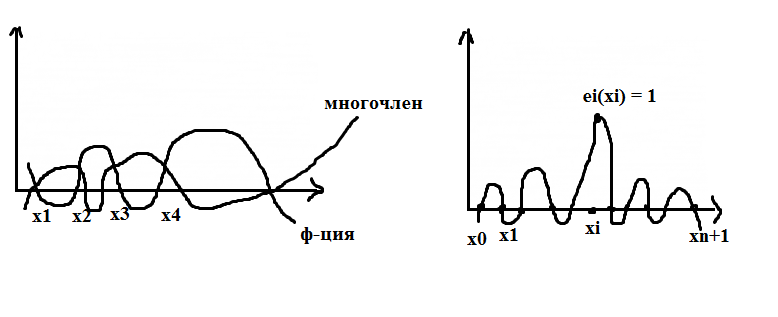
\includegraphics[scale = 0.6]{7-1.png}}
	\end{figure}\\
	$r$ непрерывно и $r$ является ретракцией $D$ на $S^1\ \Rightarrow$ противоречие предыдущему предложению, что и требовалось доказать



\newpage
%-----------------------------------------------------------------------------
	\section{}
	\textbf{Изоморфизм фундаментальной группы пространства и линейно связной компоненты отмеченной точки. Зависимость фундаментальной группы от отмеченной точки. Односвязные пространства, их эквивалентные определения (через петли и через пути). Односвязность выпуклых подмножеств $\mathbb{R}^n$}\\
	\\
	\textbf{Предложение}: $x_0, x_1 \in X,\ p\in P(x_0, x_1)$\\
	Рассмотрим ${\phi}_p: {\pi}_1(x, x_1) \rightarrow {\pi}_1(x,x_0)$\\
	${\phi}_p ([u]) = [p][u][p^{-1}]$\\
	Тогда ${\phi}_p$ -- изоморфизм групп\\
	\textbf{Доказательство}: ${\phi}_p ([u]) {\phi}_p ([v]) = [p][u][p^{-1}][p][v][p^{-1}] = [p][u][e_{x_1}][v][p^{-1}] = [p][u][v][p^{-1}] = {\phi}_p ([u][v]) \Rightarrow {\phi}_p$ -- гомоморфизм групп\\
	Заметим: ${\phi}_{p^{-1}} {\phi}_p =  \text{id}_{{\pi}_1 (X, x_1)}, {\phi}_p {\phi}_{p^{-1}} =  \text{id}_{{\pi}_1 (X, x_0)} \Rightarrow {\phi}_{p^{-1}} b {\phi}_p$ - изоморфизмы, что и требовалось доказать\\
	Нестрогое \textbf{Обозначение}: $X$ -- линейное связное топологическое пространство\\
	Фундаментальная группа $X$ -- группа ${\pi}_1 (X) \overset{опр}{ = } {\pi}_1 (X, x_0)$, где $x_0 \in X$ -- любая точка\\
	Она определена однозначно с точностью до изоморфизма (см.предложение), но не единственного\\
	\textbf{Определение}: $X$ односвязно $\Leftrightarrow X$ линейно связно и ${\pi}_1 (X)$ тривиальна\\
	Примечание: Выпуклое подномжество в нормированном пространстве односвязно\\
	\textbf{Предложение}: линейно связное топологическоепространство $X$ односвязно $\Leftrightarrow \forall x_0, x_1 \in X, \forall u, v \in P(x_0,x_1) u\simeq v$\\
	\textbf{Доказательство}:\\
	($\Rightarrow$) $[u][v^{-1}] = [e_{x_0}] \Leftrightarrow [u] = [v]$\\
	($\Leftarrow$) Взять $x_1 = x_0 и v = e_{x_0}$ что и требовалось доказать
	
	


\newpage
%-----------------------------------------------------------------------------
%6 done
	\section{}
	\textbf{Лемма о лебеговом числе. Односвязность n-мерной сферы при $ n \geq 2$}\\
	\\
	\textbf{Теорема}: $\forall n\geq 2 S^n$ односвязна (то есть ее фундаментальная группа тривиальна)\\
	\textbf{Лемма 1 (о лебеговом числе)}: $X$ -- компактное метрическое пространство, $U$ -- открытое покрытие $X \Rightarrow \exists \delta \textgreater 0$, такое что каждое $S\subset X диаметра \textless \delta$, содержится в некотором элементе $U$.\\
	\textbf{Определение}: такое $\delta$ называется лебеговым числом U\\
	\textbf{Доказательство}: $\forall x\in X$\\
	$\exists r(x) \textgreater 0$, такое что $B_{2r(x)} \subset V_x$, где $V_x\in U$\\
	Из компактности $X \Rightarrow \exists x_1,  \ldots , x_n \in X$, такое что $X = \overset{n}{\underset{i = 1}{cup}} B_{r(x_i)} (x_i)$\\
	Обозначим: $\delta = ,in \{r(x): 1 \leq i \leq n \}$\\
	Пусть $\varnothing \neq S\subset X, diam S \textless \delta$\\
	Зафиксируем: $\forall y\in S \exists i$, такое что $\phi (y,x_i) \leq r(x_i)\\
	\forall x\in S \rho (z, x_i) = \rho(z,y)+\rho(y,x_i) \textless \delta + r(x_i) \Rightarrow S\subset B_{2r(x_i)} (x_i) \subset V_{x_i}$ что и требовалось доказать\\
	\textbf{Лемма 2}: $n \leq 2, a,b, v \in S^n, c\notin \{a,b\}\\
	\forall u\in P(a,b) \exists v \in P(a,b)$, такой что $v \underset{p}{\simeq} u, v(I): c\notin v(I)$\\
	\textbf{Доказательство}: $S^n = U \cup V$, где $U$ -- окрестность $c$, гомеоморфная открытому шару в $\mathbb{R}^n$\\
	$V = S^n \diagup \{c\}$\\
	Пусть $\varepsilon$ -- лебеговое число $\{U, V\}\\
	\exists \delta \textgreater 0$, Такое что $\forall t, t\in I$, удовлетворяющее $|t-t^{\prime}| \textless \delta$, выполняется $||u(t)-u(t^{\prime})|| \textless \varepsilon$\\
	Зафиксируем разбиение: $0 = t_0 \textless t_1 \textless  \ldots  \textless t_m = 1$, такое что $t_i - t_{i-1} \textless \delta \forall i$\\
	Обозначим: $x_i = u(t_i) \in S^n$\\
	$u \underset{p}{\simeq} u_1, \ldots ,u_m$, где $u_i \in P(x_{i-1}, x_i)$, причем либо $u_i (I) \subset U$, либо $u_i (I) \subset V$\\
	$\forall i$, такой что $u_i (I) \subset U$ найдем $V_i (I) \subset U \diagup \{ c\}$ (так как $U\diagup \{c\}$ линейно связно)\\
	$u_i \underset{p}{\simeq} v_i$, так как $U$ односвязно\\
	$\Rightarrow u \underset{p}{\simeq} v$, где $v = v_1 \cdot  \ldots  \cdot v_m$, где остальные $v_i = u_i$ (по построению $c\notin V(I))$ что и требовалось доказать\\
	\textbf{Доказательство теоремы}: Пусть $a, b \in S^n, u,v \in P(a,b)$\\
	Зафиксируем: $\forall c\notin \{a,b\}$\\
	Из Леммы 2 следует, что $\exists u^{\prime},v^{\prime} \in P(a,b)$, такое что $u \underset{p}{\simeq} u^{\prime}, v \underset{p}{\simeq} v^{\prime}, c\notin u^{\prime} (I), c\notin v^{\prime} (I)\\
	S^n \diagup \{c\}$ -- гомеоморфно $\mathbb{R}^n, \mathbb{R}^n$ односвзяно $\Rightarrow u^{\prime} \underset{p}{\simeq} v_i \Rightarrow u \underset{p}{\simeq} v$ что и требовалось доказать
	


\newpage
%-----------------------------------------------------------------------------
%8 done
	\section{}
	\textbf{Фундаментальная группа произведения. Примеры: фундаментальная группа тора и фундаментальная группа $\mathbb{R}^n \diagup \{0\}$}\\
	\begin{figure}[h]
		\center{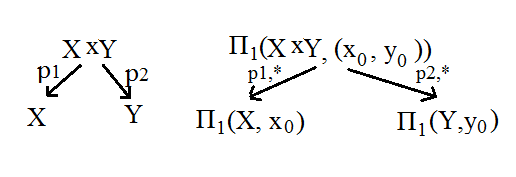
\includegraphics[scale = 0.6]{8-1.png}}
	\end{figure}\\
	$\phi: {\pi}_1 (X\times Y, (x_0,y_0)) \rightarrow {\pi}_1 (X,x_0) \times {\pi}_1 (Y,y_0)\\
	\phi (h) = (p_1, * (h) ; p_2, * (h))$\\
	\textbf{Предложение}: $\phi$ -- изоморфизм групп\\
	\textbf{Доказательство}: рассмотрим $\psi:\ {\pi}_1(X,x_0) \times {\pi}_1 (Y,y_0) \rightarrow {\pi}_1 (X\times Y, (x_0,y_0)), \psi ([u],[v]) = [(u,v,)]$, где $(u,v): I\rightarrow X\times Y, s\rightarrow (u(s), v(s))$\\
	Если $u \underset{p}{\simeq} u^{\prime}, v \underset{p}{\simeq} v^{\prime}, то (u, v) \underset{p}{\simeq} (u^{\prime}, v^{\prime})$\\
	Действительно: пусть $F: u \underset{p}{\simeq} u^{\prime}, G: v \underset{p}{\simeq} v^{\prime}$, рассмотрим $H: I\times I \rightarrow X\times Y, H_t (s) = (F_t(s), G_t (s))$\\
	$H: (u,v) \underset{p}{\simeq} (u^{\prime},v^{\prime})$, поэтому $\psi$ корректно определено\\
	Из конструкции $\phi \cdot \psi =  \text{id}, \psi \cdot \phi =  \text{id} \Rightarrow \phi$ -- изоморфизм групп\\
	\textbf{Следствие}: ${\pi}_1 (T^n, x_0) \cong \mathbb{Z}^n\\
	{\pi}_1 (T^2, x_0) = {\pi}_1 (S^1) \times {\pi}_1 (S^1)$\\
	\textbf{Следствие}: ${\pi}_1 (\mathbb{R}^n \diagup \{0\}, x_0) \cong 
	\begin{cases}
	0\ \text{если}\ n = 1\ \text{или}\ n \geq 3\\
	\mathbb{Z}\ \text{если}\ n = 2
	\end{cases}$
	\textbf{Доказательство}: $\mathbb{R} \diagup \{0\} = (-\infty,0)\sqcup(0, +\infty)$ (оба промежутка односвязны) $\Rightarrow {\pi}_1 (\mathbb{R}^n \diagup \{0\}) = 0$\\
	Пусть $n \geq 2$. рассмоторим $f: \mathbb{R}^n \diagup \{0\} \rightarrow S^{n-1} \times (0, +\infty), f(x) = (\frac{x}{||x||}, ||x||)$\\
	$f$ -- гомеоморфизм, $f^{-1} (y,t) = y\cdot t \Rightarrow {\pi}_1 (\mathbb{R}^n \diagup \{0\}, x_0) \cong {\pi}_1 (S^{n-1}) \times {\pi}_1 (0, +\infty) \cong {\pi}_1 (S^{n-1}) \cong
	\begin{cases}
	0\ \text{если}\ n = 1\ \text{или}\ n \geq 3\\
	\mathbb{Z}\ \text{если}\ n = 2
	\end{cases}$
	


\newpage
%-----------------------------------------------------------------------------
%10 done 
\section{}	
	\textbf{Гомотопическая эквивалентность и ее категорная интерпретация. Деформационные ретракции и строгие деформационные ретракции. Сфера $S^n$ как строгий деформационный ретракт $\mathbb{R}^n \diagup \{0\}$. Биекция ${\pi}_0 (X) \cong [pt, X]$. Следствие: гомотопическая инвариантность свойства линейной связности. Стягиваемые пространства, их эквивалентные определения, примеры.}\\
	\textbf{Определение}: $X, Y$ -- топологические пространства. Непрерывное $f: X \rightarrow Y$ -гомотопическая эквивалентность $\Leftrightarrow$ существует непрерывное $g: Y \rightarrow X$, такое что $f \circ g \simeq  \text{id}_Y, g \circ f \simeq if_X. g$ называется гомотопически обратным к $f$.\\
	$X$ и $Y$ гомотопически эквивалентны $(X\simeq Y) \Leftrightarrow$ существует гомотопическая эквивалентность $X\rightarrow Y$\\
	\textbf{Наблюдение}: гомеоморфизм является гомотопической эквивалентностью\\
	Обозначим гомотопической категорией $Hmt: \text{Ob}(Hmt)$ -- топологические пространства\\
	Морфизмы -- гомотопические классы непрерывных отображений $\text{Hom}_Hmt (X,Y) = [X,Y] = {C(X,Y)\diagup}_{\simeq}, [g]o[f] = [g \circ f]$\\
	\textbf{Наблюдение}: $f: X\rightarrow Y$ -- гомотопическая эквивалентность $\Leftrightarrow$ его гомотопический класс -- изоморфизм в $Hmt$\\
	Следствие: 
	\begin{enumerate}
		\item $f: X\rightarrow Y,\ g: Y \rightarrow Z$ -- гомотопические эквивалентности $\Rightarrow g \circ f$ -- гомотопическая эквивалентность
		\item Если $f: X\rightarrow Y$ -- гомотопическая эквивалентность, $g: Y\rightarrow$ -- его гомотопически обратный	
	\end{enumerate}
	Непрерывный $g_1: Y \rightarrow X$ гомотопические обратно к $f \Rightarrow g_1 \simeq g$\\
	\textbf{Определение}: $X$ -- топологическоепространство, $A\subset X$. Ретракция $r X$ на $A$ (то есть непрерывное $r: X\rightarrow A$, такое что $r \circ i_A =  \text{id}_A$) называется:\\
	\begin{enumerate}
		\item Деформационной ретракцией $\Leftrightarrow i_A \circ r \simeq  \text{id}_X$
		\begin{figure}[h]
			\center{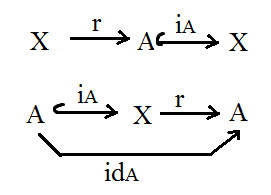
\includegraphics[scale = 0.6]{10-1.png}}
		\end{figure}
		\item строгой деформационной ретракцией $\Leftrightarrow i_a \circ r \underset{A}{\simeq} if_X$\\
		$A$ называется деформационным ретрактом( соответственно строгим деформационным ретрактом) $X \Leftrightarrow$ существует деформационная ретракция (соответственно строгая днформационная ретракция) $X$ на $A$
	\end{enumerate}
	Строгая деформационная ретракция $\Rightarrow$ деформационная ретракция $\Rightarrow$ ретракция\\
	\textbf{Наблюдение}: деформационная ретракция является гомотопической эквивалентностью\\
	\textbf{Предложение}: $S^n$ -- строгий деформационнный ретракт $\mathbb{R} \diagup \{0\}$\\
	\textbf{Доказательство}: рассмотрим ретракцию $r: \mathbb{R}^{n+1} \diagup \{0\} \rightarrow S^n$\\
	$r(x) = \frac{x}{||x||}$\\
	Рассмотрим $F: \mathbb{R}^{n+1} \diagup \{0\} \times I \rightarrow \mathbb{R}^{n+1} \diagup \{0\}\\
	F(x,t) = t \frac{x}{||x||} + (1-t)x\\
	F_0 =  \text{id}, F_1 = i_{S^n} \circ r \Rightarrow r$ -- строгая деформационная ретракция что и требовалось доказать\\
	Терминология: гомотопические свойства топологические пространства -- свойства, которые сохраняются при гомотопических эквивалентностях\\
	\textbf{Обозначение}: $pt = \{p_0\}$ -- топологические пространство, состоящее из одной точки $p_0$\\
	\textbf{Обозначение}: $X$ -- топологические пространство, ${\pi}_0 (X)$ -- множество его линейно связных компонент\\
	\textbf{Предложение}: для любого топологические пространства X существует биекция $[pt,X] \rightarrow {\pi}_0 (X), [f] \rightarrow PC (f(p_0))$ -- линейно связная компонента $f(p_0) (*)$\\
	\textbf{Доказательство}: Заметим: отображение $C(pt, X) \rightarrow X\\
	f\rightarrow f(p_0)$ -- биекция\\
	Пусть $f,g: pt \rightarrow x, F: f\simeq g$\\
	$F$ порождает путь $u\in P(f(p_0), g(p_0)), u(t) = F(p_0, t)$\\
	Наоборот: кадлый путь $u\in P(f(p_0), g(p_0))$ порождает $F: f\simeq g$\\
	Поэтому: $f\simeq g \Leftrightarrow f(p_0) и g(p_0)$ лежат в одной линейно связной компоненте $\Rightarrow$ отображение (*) корректно определенно и является биекцией что и требовалось доказать\\
	Следствие: $X\simeq Y, Y$ -- линейно связно $\Rightarrow Y$ линейно связно\\
	\textbf{Доказательство}: $X \cong Y в Hmt$\\
	$[pt, -]$ -- ковариантный функтор $Hmt \rightarrow Sets$ (частный случай $\text{Hom}$ -- функтора) $\Rightarrow [pt, X]( = {\pi}_0 (X)) \cong [pt,Y] ( = {\pi}_0 (Y)) в Sets \Rightarrow {\pi}_0 (Y)$ одноэлементно, то есть $Y$ -линейно связно что и требовалось доказать\\
	\\
	\textbf{Стягиваемые пространства, их эквивалентные определения, примеры.}\\
	\textbf{Определение}: топологическоепространство $X$ стягиваемо $\Leftrightarrow X \simeq pt$\\
	\textbf{Наблюдение}: Стягиваемость -- гомотопическое свойство, стягиваемость $\Rightarrow$ линейная связность\\
	\textbf{Теорема}: следующие свойства топологические пространства $X\neq \varnothing$ эквивалентны:\\
	\begin{enumerate}
		\item $X$ -- стягиваемо
		\item (2)для любого $Y$ -- топологические пространства любые два непрерывных $f,g: Y \rightarrow X$ гомотопны
		\item $\exists x_0 \in X$, такое что $ \text{id}_X \simeq C_{x_0}$ (где $C_{x_0}: X\rightarrow X, C_{x_0} (x) = x_0 \forall x\in X$)
		$^{\prime}\quad \exists x_0 \in X$, такое что $\{x_0\}$ -- деформационный ретракт X
		\item $\forall x_0 \in X if_X \simeq C_{x_0}$
		$^{\prime}\quad \forall x_0 \in X \{x_0\}$ -- деформационный ретракт $X$
	\end{enumerate}
	\textbf{Доказательство}:\\
	$(3) \Leftrightarrow (3^{\prime})$ и $(4)\Leftrightarrow (4^{\prime})$ из определения деформационного ретракта.\\
	Действительно: ретракция $X$ на $\{x_0\}$ -отображение $r_{x_0}: X \rightarrow \{x_0\} r_{x_0} (x) = x_0 \forall x$\\
	Она дефракционный ретракт $\Leftrightarrow i_{\{x_0\}} \circ r_{x_0}( = C_{x_0}) \simeq if_X$\\
	\\
	$(1)\Rightarrow (2)$: $[Y, -]: Hmt \rightarrow Sets$ -- функтор (частный случай $\text{Hom}$ -- функтора)\\
	$X \cong pt в Hmt \Rightarrow [Y,X]$ и $[Y, pt]$ равномощны, но $[Y, pt]$ состояит из одной точки $\Rightarrow [Y,X]$ -- тоже\\
	\\
	$(2) \Rightarrow (4) \Rightarrow (3)$ -- очев\\
	\\
	$(3) \Rightarrow (1)$ $X \overset{f}{\rightarrow} pt \overset{g}{\rightarrow} x, pt = \{p_0\}\\
	f(x) = p_0 \forall x\in Y, g(p_0) = x_0\\
	g \circ f = C_{x_0} \simeq if_X\\
	f \circ g =  \text{id}_{pt}\\
	\Rightarrow f$ -- гомотопическая эквивалентность что и требовалось доказать\\
	\textbf{Наблюдение}: для любого топологические пространства $X \forall x_0 \in X \{x_0\}$ -- ретракт $X$\\
	С другой стороны $\{x_0\}$ -- деформационный ретракт $\Leftrightarrow X$ -- стягиваемое\\
	Поэтому ретракт не всегда является деформационным ретрактом\\
	Пример: $X$ -- нормальное пространство, $Y\subset X$ -- звездное относительно $x_0 \in Y$. Тогда $Y$ -- стягиваемое\\
	Действительно: $F(x,t) = tx_0 + (1-t)x$ -- гомотопия между $ \text{id}_Y$ и $C_{x_0}$
	


\newpage
%-----------------------------------------------------------------------------
%16 done 
\section{}
	\textbf{Стабилизатор точки при действии группы. Сопряженность стабилизаторов точек из одной орбиты. Морфизмы G-множеств. Изоморфизм между орбитой и множеством смежных классов по стабилизатору. Гомоморфизм фундаментальных групп, индуцированный накрывающим отображением: его мономорфность и описание его образа как стабилизатора точки слоя. Следствие: изоморфизм между слоем накрытия и множеством смежных классов фундаментальной группы базы накрытия.}\\
	\\
	$G$ -- группа, $X$ -- правое $G$ -множество\\
	\textbf{Определение}: Стабилизатор точки $x\in X$ -- это $\text{Stab}(x) = \{g\in G| x\cdot g = x\} \subset G$\\
	Синонимы: стационарная подгруппа, подгрупппа изотропии\\
	\textbf{Наблюдение}: $\text{Stab}(x) \textless G$\\
	\textbf{Определение}: Правое действие $G$ на $G$ сопряжениями задается формулой: $x\ast g = g^{-1} xg (x,g\in G)$. Аналогично определяются действия сопряжениями на множестве подгрупп в $G: H\ast g = g^{-1} Hg = \{g^{-1} hg|h\in H\}$\\
	$X$ -- правое $G$-множество\\
	\textbf{Предложение}: стабилизаторы точек из одной орбиты сопряжены друг другу.\\
	Более точно: $\text{Stab}(x\cdot g) = g^{-1} \text{Stab}(x) \cdot g$\\
	Доказательство $h\in \text{Stab}(x\cdot g) \Leftrightarrow x\cdot g\cdot h = h\cdot g \Leftrightarrow x\cdot g\cdot h\cdot g^{-1} = x \Leftrightarrow g\cdot h\cdot g^{-1} \in \text{Stab}(x) \Leftrightarrow h\in g^{-1} \text{Stab}(x) g$\\
	\textbf{Определение}: $X, Y$ -- правые $G$-множества\\
	Отображение $\phi:\ X\rightarrow Y$ -- морфизм $G$-множеств ($G$-эквивалентное отображение) $\Leftrightarrow \phi (x\cdot g) = \phi (x) \cdot g (x\in X, g\in G$)\\
	Правые $G$-множества и их морфизм образуют категорию. Обозначают ее $G-Sets$\\
	\textbf{Предложение}: $X$ -- правое $G$-множество, $x\in X, x\in X$. Существует изоморфизм правых $G$-множеств\\
	$\phi:\ {G\diagup}_{\text{Stab}(X)} \overset{\sim}{\rightarrow} x\cdot G, \phi(\text{Stab}(x)\cdot g) = x\cdot g (g\in G)$.\\
	В частности, если $X$ транзитивно, то $\phi$-изоморфизм ${G\diagup}_{\text{Stab}(X)}$ на $X$.\\
	\textbf{Доказательство}: пусть $g, h \in G$\\
	$\text{Stab}(x)\cdot g = \text{Stab}(x)\cdot h \Leftrightarrow g\cdot h^{-1} \in \text{Stab}(x) \Leftrightarrow x\cdot g\cdot x^{-1} = x\Leftrightarrow x\cdot g = x\cdot h$\\
	Поэтому $\phi$ -- корректно определенно и инъективно. Очевидно, $\phi$ -- сюръективно и является морфизмом G-множеств что и требовалось доказать\\
	Гомоморфизм фундаментальных групп, индуцированный накрывающих отображением.\\
	$p: E\rightarrow X -- накрытие, x_0 \in X, a\in p^{-1} (x_0)\\
	p_x: {\pi}_1 (E, a) \rightarrow {\pi}_1 (X, x_0)$\\
	Напоминания: Пусть $x_1\in X, u\in P(x_0,x_1), \overset{\sim}{u_a}$ -- поднятие $u$, такое что $\overset{\sim}{u_a} (0) = a$ (оно существует и единственное)\\
	Если $v,u\in P(x_0,x_1)$, то $u \underset{p}{\simeq} v \Leftrightarrow \overset{\sim}{u_a} \underset{p}{\simeq} \overset{\sim}{v_a} \Rightarrow \overset{\sim}{u_a} (1) = \overset{\sim}{v_a} (1)$\\
	\begin{figure}[h]
		\center{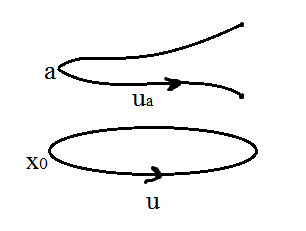
\includegraphics[scale = 0.6]{16-1.png}}
	\end{figure}\\
	Действие монодромии: $p^{-1} (x_0) \times {\pi}_1 (X, x_0) \rightarrow p^{-1} (x_0), (a,[u])\rightarrow a[u] = \overset{\sim}{u_a} (1)$\\
	\textbf{Теорема}: $p: E\rightarrow X$ -- накрытие, $x_0 \in X, a\in p^{-1} (x_0)$
	\begin{enumerate}
		\item $p_{\ast}:\ {\pi}_1 (E,a) \rightarrow {\pi}_1 (X,x_0)$ -- мономорфизм
		\item $Im p_{\ast} = \{ [u]:\ \overset{\sim}{u_a}$ -- петля$\}$
		\item $Im p_{\ast} = \text{Stab}(a)$ при действии монодромии
		\begin{figure}[h]
			\center{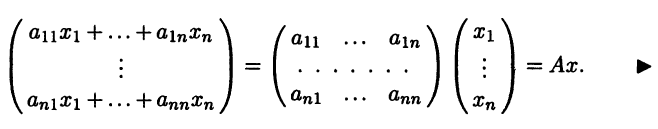
\includegraphics[scale = 0.6]{16-2.png}}
		\end{figure}
	\end{enumerate}
	\textbf{Доказательство}:
	\begin{enumerate}
		\item Пусть $[v] \in Ker p_{\ast}$. Обозначим $u = p\cdot v$\\
		$u \underset{p}{\simeq} e_{x_0} \Rightarrow \overset{\sim}{u_a} \underset{p}{\simeq} {(\overset{\sim}{e_{x_0}})}_a ( = e_a), то есть [v] = [e_a] \in {pi}_1 (E,a)$
		\item $[u]\in Im p_{\ast} \Leftrightarrow u \underset{p}{\simeq} p \circ v$ для некоторой петли $v$ в $a \Leftrightarrow \overset{\sim}{u_a} \underset{p}{\simeq} v$ для некоторой петли $v$ в $a \Leftrightarrow \overset{\sim}{u_a}$ -- петля
		\item $\overset{\sim}{u_a} -петля \Leftrightarrow \overset{\sim}{u_a} (1) = a \Leftrightarrow a = a\cdot [u] \Leftrightarrow [u] \in St(a)$ что и требовалось доказать
	\end{enumerate}
	\textbf{Следствие}: $p: E\rightarrow X$ -- накрытие\\
	$E$ -- линейно связно, $x_0 \in X, a\in p^{-1} (x_0)$. Существует изоморфизм правых ${\pi}_1 (X,x_0)$ -- множеств\\
	${{\pi}_1 (X,x_0) \diagup}_{Im p_{\ast}} \overset{\sim}{\rightarrow} p^{-1} (x_0), (Im p_{\ast})\cdot [u] \rightarrow a\cdot [u] = \overset{\sim}{u_a} (1)$\\
	\textbf{Доказательство}: из п.(3) теоремы и транзитивности монодромии что и требовалось доказать
		
	
	
\newpage
%-----------------------------------------------------------------------------
%13 done 
	\section{} 
	\textbf{Накрытия. Примеры накрытий. Число листов накрытия, его независимость от выбора точки базы (если последняя связна). Теорема о единственности поднятия.}\\
	X -- топологическоепространство
	\\
	\textbf{Определение}: Накрытие $X$ -- пара $(E, p)$, где $E$ -- топологические пространство, $p: E \rightarrow X$ непрерывно, такое что: $\forall x\in X$ существует окрестность $U \ni U$, такая что $p^{-1} (U) = \underset{i\in I}{\sqcup} U$ (достаточно потребовать дизъюнктное отбъединение множеств), $(I \neq \varnothing)$, где $U_i$ открыто $\forall i$, и ${p|}_{U_i)}$ -- гомеоморфизм $U_i$ на $U$.\\
	$X$ называется базой накрытия, $E$ -- накрывающее пространство, $p$ -- накрывающее отображение. Часто само $p$ называют накрытие.\\
	$\forall x\in X$ множество $p^{-1} (X)$ называется слоем над $X$.\\
	\textbf{Наблюдение}: $(E,p)$ накрытие $\Rightarrow p$ -- сюръекция $E$ на $X$\\
	\\
	\textbf{Пример 1}: любой гомеоморфизм является накрытием\\
	\textbf{Пример 2}: $X$ -- топологическоепространство, $D$ -- дискретное пространство. $p: X\times D, p(x, в) = x$ -- накрытие\\
	Действительно: $\forall U \subset X p^{-1} (U) = U\times D = \underset{d\in D}{\sqcup} (U \times \{ d\})$ (открыто в $X\times D$, так как $D$ -- дискретно)\\
	\textbf{Пример 3}: $p: \mathbb{R} \rightarrow S^1, p(t) = e^{2\pi it}$ -- накрытие\\
	Действительно: для любого отрезка $I\subset \mathbb{R}$ длины меньше 1\\
	${p|}_I:\ I \rightarrow p(I)$ -- гомеоморфизм\\
	(т.к. $I$ -- компактно, $p|{I}$ -- инъективно) $\Rightarrow$ для любого интревала $J \subset \mathbb{R}$ длины меньше 1 множество $U = p(J)$ открыто в $S^1, p^{-1} (U) = \underset{n\in \mathbb{Z}}{\sqcup} J_n$, где $J_n = J_n, J_n$ -- интервал, ${p|}_{J_n} \rightarrow U$ -- гомеоморфизм\\
	Вся $S^1$ покрывается двумя такими $U \Rightarrow p$ -- накрытие\\
	\textbf{Предложение}: $p: E\rightarrow X, q: F\rightarrow Y$- накрытия $\Rightarrow p\times q:\ E\times F \rightarrow X\times Y$ -- накрытие\\
	\textbf{Доказательство}: очев\\
	\textbf{Пример 4}: $p: \mathbb{R}^n \rightarrow T^n p(t_1, \ldots , t_n) = (e^{2\pi it_1},  \ldots , e^{2\pi it_n})$ -- накрытие\\
	\textbf{Пример 5}: $\mathbb{R} \mathbb{P}^n = S^n {\diagup}_{\sim}, где x\sim y \Leftrightarrow x = \pm y$\\
	Отображение факторизации $q: S^n \rightarrow \mathbb{R} \mathbb{P}^n$ -- накрытие\\
	Действительно: для любого открытого $U\subset S^n$, такое что $\overline{U}$ не содержит диаметрально противоположных точек, ${q|}_{\overline{U}}: \overline{U} \rightarrow q(\overline{U})$ -- гомеоморфизм (так как ${q|}_{\overline{U}}$ -- инъекция, $\overline{U}$ компакт) $\Rightarrow q(U)$ открыто в $\mathbb{R} \mathbb{P}^n, q^{-1} (U) = U \sqcup (-U)$ ($U$ и $-U$ открыты) (если $U \cap (-U) = \varnothing$)\\
	${q|}_{\pm U}: \pm U \rightarrow q(U)$ -- гомеоморфизм\\
	\textbf{Определение}: непрерывное $f: X\rightarrow Y$ локальный гомеоморфизм $\Leftrightarrow \forall x\in X$ существует окрестность $U\ni x$, такая что $f(U)$ открыто в $Y$ и ${f|}_U: U \rightarrow f(U)$ -- гомеоморфизм\\
	\textbf{Наблюдение}: накрытие является локальным гомеоморфизмом\\
	Предл: $p: E\rightarrow X$ -- накрытие, $X$ -- связно $\Rightarrow \forall x,y\in X p^{-1} (x)$ и $p^{-1} (y)$ равномощны\\
	\textbf{Доказательство}: введем на $X$ отношение эквивалентности: $x\sim y \Leftrightarrow p^{-1} (x) и p^{-1} (y)$ равномощны\\
	Достаточно докащать: $\forall x\in X$ ее $[x]$ открыт в $X$\\
	Выберем окрестность $U\ni x$, такая что $p^{-1} (U) = \underset{i\in I}{\sqcup} U_i$, гомеоморфизм ${p|}_{U_i}: U_i \rightarrow U$\\
	Заметим: $\forall y \in U p^{-1} (y) \cap U_i$ состят ровно из одной точки $(\forall i \in I)\ \Rightarrow p^{-1} (y)$ и $I$ равномощны $\Rightarrow U \subset [x] \Rightarrow [x]$ -- открыт что и требовалось доказать\\
	\textbf{Определение}: Пусть $p: E\rightarrow X$, $X$ -- связно. Числом листов этого накрытия называют мощность $p^{-1} (x) (\forall x\in X)$\\
	Пример: накрытие из примера 5 двулистно, из примеров 3, 4 -- счетно листно\\
	\textbf{Определение}: $E, X, Y$ -- топологические пространства, $p: E\rightarrow X, f: Y\rightarrow X$ -- непрерывные. Непрерывное $g: Y\rightarrow E$ -- поднятие(относительно $p) \Leftrightarrow pog = f$\\
	\begin{figure}[h]
		\center{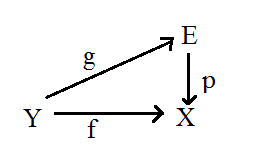
\includegraphics[scale = 0.6]{13-1.png}}
	\end{figure}\\
	\textbf{Теорема}: $p: E \rightarrow X$ -- накрытие, $f: Y\rightarrow X, Y$ -- связно, $g_1, g_2: Y \rightarrow E$ -- поднятие $f$. Пусть $\exists y_0 \in Y$, такой что $g_1 (y_0) = g_2 (y_0) \Rightarrow g_1 = g_2$ (единственность поднятия)\\
	\textbf{Лемма}: $p: E \rightarrow X$ -- накрытие, $D = \{ (x,x)|x\in E\} \subset E\times E$\\
	$Z = \{(x,y) \in E\times E | p(x) = p(y)\}$\\
	Тогда $D$ открыто и замкнуто в $Z$\\
	\textbf{Замечание}: $E$ хаусдорфово $\Leftrightarrow D$ замкнуто в $E\times E \Rightarrow$ в $Z$ тоже\\
	\textbf{Доказательство леммы}: Пусть $(x,x)\in D$, существует окрестность $U\ni x$, такая что ${p|}_U: U \rightarrow p(U)$ -- гомеоморфизм $\Rightarrow (U\times U) \cap Z$ -- окрестность $(x,x) в Z$\\
	$(U\times U)\cap Z \subset D \Rightarrow D$ -- открыт в $Z$\\
	Если $(y_1,y_2) \in (U\times U)\cap Z$, то $y_1,y_2 \in U и p(y_1) = p(y_2) \Rightarrow y_1 = y_2$, то есть $(y_1,y_2)\in D$\\
	Пусть $(x,y)\in Z\diagup D$, выберем окрестность $V\subset X$ точки $p(x) = p(y)$, такая что $p^{-1} (V) = \underset{i\in I}{\sqcup} V_i, V_i$ -- открыто\\
	${p|}_{V_i}: V_i \rightarrow V$ -- гомеоморфизм\\
	$\exists i,j \in I$, такие что $x\in V_i, y\in V_j$, причем $i\neq j$(так как $x\neq y$)\\
	$W = (V_i \times V_j) \cap Z$ -- окрестность $(x,y) в Z$\\
	$W \cap D = \varnothing$ (так как $V_i \cap V_j = \varnothing$) $\Rightarrow Z\diagup D$ открыто в $Z$, то есть $D$ замкнуто в $Z$ что и требовалось доказать\\
	\textbf{Доказательство теоремы}: Рассмотрим $g: Y\rightarrow Z, g(y) = (g_1 (y), g_2 (y)), g$ непрерывно $\Rightarrow g^{-1} (D)$ открыто и замкнуто в $Y, g^{-1} (D) = Y$, то есть $g_1 = g_2$ что и требовалось доказать
	


\newpage
%-----------------------------------------------------------------------------
%14 done
\section{}
	\textbf{Теорема о накрывающей гомотопии. Следствие: теорема о поднятии путей. Теорема о поднятии гомотопий путей.}\\
	\\
	\textbf{Теорема о накрывающей гомотопии}: $p: E \rightarrow X$ -- накрытие, $Y$ -- топологические пространство, $F: Y\times I \rightarrow X$ -- непрерывно, $f: Y \rightarrow E$ -- поднятие $F_0$ (где $F_0 Y\rightarrow X F_0 (y) = F(y,0))$\\
	Тогда существует единственное непрерывное $\overset{\sim}{F}:\ Y\times I \rightarrow E$, поднимающее $F$ и такое, что $\overset{\sim}{F_0} = f$\\
	Если, кроме того, $F -- A$-гомотопия для некоторого $A\subset Y$, то и $\overset{\sim}{F} -- A$-гомотопия\\
	Обозначения: пусть $F: Y\times \rightarrow X \forall t\in I F_t:\ Y\rightarrow X, F_t (y) = F(y,t)$\\
	$\forall y \in Y F^y:\ I\rightarrow X, F^y (t) = F(y,t)$\\
	\textbf{Лемма (о локальном поднятии)}:\\
	Пусть выполняются условия теоремы, и пусть все пространство $X$ ровно накрыто (то есть $p^{-1} (x) = \underset{i\in I}{\sqcup} U_i, U_i$ открыто в $E$, такое что ${p|}_{U_i}: U_i \rightarrow X$ -- гомеоморфизм). Тогда $\forall y\in Y$ существует окрестность $Z \ni y$ и поднятие $\overset{\sim}{F}: Z\times I \rightarrow E$ отображения ${F|}_{Z\times I}$, такое что $\overset{\sim}{F_0} = {f|}_Z$\\
	\textbf{Доказательство}: $\forall y\in Y$ существует окрестность $U\subset E$, такая что ${p|}_U:\ U\rightarrow X$ -- гомеоморфизм и $f(y)\in U$. Положим $Z = f^{-1} (U)$\\
	Обозначим $S = ({p|}_U)^{-1}: X\rightarrow U$, рассмотрим $\overset{\sim}{F}: Z\times I \rightarrow E, \overset{\sim}{F} = S \circ {F|}_{Z\times I}$\\
	$pS =  \text{id}_x \Rightarrow \overset{\sim}{F}$ -- поднятие ${F|}_{Z\times I}$\\
	$\forall z\in Z f(z) \in U \overset{\sim}{F_0} (z) \in U, p(f(z)) = F_0 (z) = p(\overset{\sim}{F_0} (z)) \Rightarrow f(z) = \overset{\sim}{F_0} (z)$, то есть $\overset{\sim}{F_0} = {f|}_Z$ что и требовалось доказать\\
	\textbf{Следствие из теоремы (о поднятии путей)}: $p: E\rightarrow X$ -- накрытие, $x_0 \in X, y\in P^{-1} (x_0)$. Тогда для любого пути $u: I\rightarrow X$, такого что $u(0) = x_0$, существует единственный путь $\overset{\sim}{u}:\ I \rightarrow E$, поднимающий $u$, такой что $\overset{\sim}{u} (0) = y$\\
	\textbf{Доказательство теоремы}: применить теорему для $Y = pt$ что и требовалось доказать\\
	\\
	Теорема (о поднятии гомотопий путей): $p: E \rightarrow X$ -- накрытие, $x_0, x_1 \in X, y\in p^{-1} (x_0), u,v\in P(x_0,x_1)\\
	\overset{\sim}{u}, \overset{\sim}{v}: I \rightarrow E$ -- поднятия $u,v$, такие что $\overset{\sim}{u} (0) = \overset{\sim}{u} (0) = y$ (они существуют и единственны по утверждению о поднятии путей).\\
	Тогда:
	\begin{enumerate}
		\item каждая гомотопия $F: u \underset{\simeq}{p} v$ единственным образом поднимается до $\overset{\sim}{F}: \overset{\sim}{u} \underset{\simeq}{p}\overset{\sim}{v}$\\
		\item $ u \underset{\simeq}{p} v \Rightarrow \overset{\sim}{u} \underset{\simeq}{p}\overset{\sim}{v}$\\
		\item Если $u \underset{p}{\simeq} v, то \overset{\sim}{u} (1) = \overset{\sim}{v} (1)$\\
		\begin{comment}
		\begin{figure}[h]
		\center{\includegraphics[w \text{id}th = 0.6\linew \text{id}th]{15-1.png}}
		\end{figure}\\
		\end{comment}
	\end{enumerate}
	\textbf{Доказательство}:\\ 
	\\
	(1) по теореме о накрывающей гомотопии, существует единственное непрерывное $\overset{\sim}{F}: I\times I \rightarrow E$, поднимающее $F$ и $\overset{\sim}{F_0} = \overset{\sim}{u_0}$\\
	Кроме того, $\overset{\sim}{F}$ (как и $F$) -- $\{0,1\}$-гомотопия (то есть гомотопия путей)\\
	$\overset{\sim}{F_1}$ -- поднятие $F_1 = v, \overset{\sim}{F_1} (0) = \overset{\sim}{F_0} (0) = \overset{\sim}{u} (0) = y$\\
	(все пути начинаются и заканчиваются в одной точке)\\
	Из единственности следует, что $\overset{\sim}{F_1} = \overset{\sim}{v}$, то есть $\overset{\sim}{F}: \overset{\sim}{u} \underset{p}{\simeq}\overset{\sim}{v}$\\
	\\
	(2)($\Rightarrow$) Из (1)\\
	($\Leftarrow$ ) Пусть $G: \overset{\sim}{u} \underset{p}{\simeq}\overset{\sim}{v} \Rightarrow poG: u \underset{p}{\simeq} v$\\
	\\
	(3) Из (2) что и требовалось доказать\\



\newpage
%-----------------------------------------------------------------------------
\section{}
	\textbf{Отображение фундаментальной группы базы накрытия в слой над отмеченной точкой; условия его сюръективности и биективности. Фундаментальная группа вещественного проективного пространства.
}\\
	\\	
	Обозначим: $z = y\cdot [u] = \overset{\sim}{u_y} (1) \Rightarrow (y [u]) \cdot [v] = z \cdot [v] = \overset{\sim}{v_z} (1)\\
	\overset{\sim}{u_y} \cdot \overset{\sim}{v_z}$ -- поднятие $u\cdot v$\\
	$(\overset{\sim}{u_y} \cdot \overset{\sim}{v_z}) (0) = \overset{\sim}{u_y} (0) = y \Rightarrow \overset{\sim}{u_y} \cdot \overset{\sim}{v_y} = \overset{\sim}{(uv)_y}\\
	y\cdot ([u][v]) = y[u\cdot v] = \overset{\sim}{(uv)_y} (1) = (\overset{\sim}{u_y} \cdot \overset{\sim}{v_z}) (1) = \overset{\sim}{v_z} (1) \Rightarrow (y\cdot [u])[v] = y([u][v]) \Rightarrow (*)$ определяет действие\\
	\begin{comment}
	\begin{figure}[h]
	\center{\includegraphics[scale = 0.6]{15-3.png}}
	\end{figure}\\
	\end{comment}
	Пусть $E$ линейно связно, $y,z \in p^{-1} (x_0)$\\
	Выберем $v \in P(y,z)$, обозначим $u = p\cdot v \Rightarrow u$ -- петля в $x_0, v = \overset{\sim}{u_y} \Rightarrow y\cdot [u] = v(1) = z \Rightarrow$ действие транзитивно\\
	Пусть $E$ односвязно, $y\in p^{-1} (x_0), [u]\in {\pi}_1 (X,x_0), y[u] = y$, то есть $y = \overset{\sim}{u_y} (1) \Rightarrow \overset{\sim}{u_y}$ -- петля в $y \Rightarrow \overset{\sim}{u_y} \simeq e_y \Rightarrow u \underset{p}{\simeq} e_{x_0}$, то есть $[u] = [e_{x_0}] \Rightarrow$ действие свободно что и требовалось доказать\\
	Следствие: $p: E\rightarrow X$ -- накрытие, $E$ -- односвязно $\Rightarrow \forall x_0 \in X, \forall y\in p^{-1} (x_0)$, отображение ${\pi}_1 (x,x_0) \rightarrow p^{-1} (x_0), [u] \rightarrow y[u]$ -- биекция\\
	Пример: Пусть $p: \mathbb{R}
	\rightarrow S^1, p(t) = e^{2\pi it}, x_0 = 1 \in S^1, y = 0 \in p^{-1} (1) = \mathbb{Z}$\\
	Отображение ${\pi}_1 (S^1, 1) \rightarrow \mathbb{Z}$ из предыдущего следствия действие по формуле $[u] \rightarrow \text{deg}(u)$\\
	Следствие: ${\pi}_1 (\mathbb{RP}^n, x_0) \simeq {\mathbb{Z}\diagup}_{2\mathbb{Z}} \forall n \geq 2 \forall x_0 \in \mathbb{RP}^n$\\
	\textbf{Доказательство}: знаем отображение факторизации $q: S^n \rightarrow \mathbb{RP}^n$ -- двулистное накрытие, $S^n$ -- односвязно $\Rightarrow$ (по предыдущему следствию) существует биекция ${\pi}_1 (\mathbb{RP}^n, x_0) \cong q^{-1} (x_0)\\
	q^{-1} (x_0)$ -- из 2 элементов $\Rightarrow {\pi}_1 (\mathbb{RP}^n, x_0) \simeq {\mathbb{Z}\diagup}_{2\mathbb{Z}}$ что и требовалось доказать\\


\newpage
%-----------------------------------------------------------------------------
	\section{}
	\textbf{Гомоморфизм фундаментальных групп, индуцированный накрывающим отображением: его мономорфность и описание его образа. Критерий существования поднятия отображения, действующего в базу накрытия, до отображения в накрывающее пространство. Следствие: существование и единственность поднятия отображения из односвязного пространства.
}\\
	\\	
	Общая теорема о поднятии\\
	\begin{figure}[h]
		\center{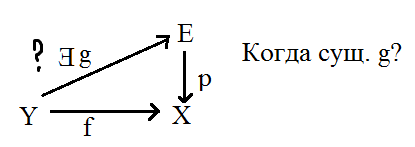
\includegraphics[scale = 0.6]{17-1.png}}
	\end{figure}\\
	Видоизменим задачу\\
	$y_0 \in Y, x_0 = f(y_0), a_0 \in p^{-1} (x_0)$. Когда существует поднятие $g$, такое что $g(y_) = a_0$?\\
	\begin{figure}[h]
		\center{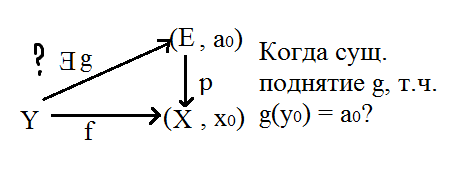
\includegraphics[scale = 0.6]{17-2.png}}
	\end{figure}\\
	Применим функтор:\\
	\begin{figure}[h]
		\center{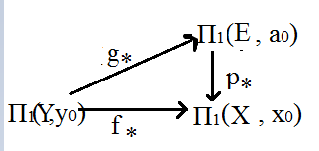
\includegraphics[scale = 0.6]{17-3.png}}
	\end{figure}\\
	$p_{\ast} \circ g_{\ast} = f_{\ast} \Rightarrow Im f_{\ast} \subset Im p_{\ast}$\\
	\textbf{Наблюдение}: Если существует поднятие $g: Y\rightarrow E$ отображения $f: Y\rightarrow X$, такое что $g(y_0) = a_0 \Rightarrow Im f_{\ast} \subset Im p_{\ast}$\\
	\textbf{Определение}: топологическоепространство $Y$ локально линейно связно $\Leftrightarrow \forall y\in Y$ для любой окрестности $U\ni y$ существует линейно свячзная окрестность $V\ni y V\subset U$\\
	\textbf{Напоминание}: открытое подмножество любого нормированного пространства локально линейно связно\\
	\textbf{Напоминание}: $Y$ связно, $U$ локально линейно связно $\Rightarrow Y$ линейно связно\\
	\textbf{Теорема}: $p: E\rightarrow X$ -- накрытие, $z_0 \in X, a_0 \in p^{-1} (x_0)$\\
	$f: Y \rightarrow X, f(y_0) = x_0$\\
	\textbf{Предположим}: $Y$ связно и локально линейно связно $\Rightarrow$ следующие утверждения эквивалентны:
	\begin{enumerate}
		\item существует поднятие $g: Y\rightarrow E$ отображения $f$, такое что $g(y_0) = a_0$
		\item $Im (f_{\ast}: {\pi}_1 (Y,y_0) \rightarrow {\pi}_1 (X,x_0)) \subset Im(p_{\ast}: {\pi}_1 (E,a_0) \rightarrow {\pi}_1 (X,x_0))$
	\end{enumerate}
	\textbf{Доказательство}: (1) $\Rightarrow$ (2) см.выше\\
	(2) $\Rightarrow$(1) $Y$ линейно связно. $\forall y\in Y выберем u\in P(y_0,y)$\\
	\begin{figure}[h]
		\center{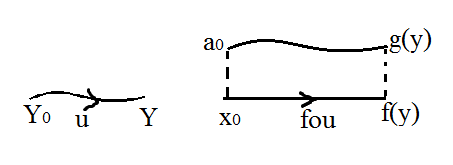
\includegraphics[scale = 0.6]{17-4.png}}
	\end{figure}\\
	Положим $g(y) = (fou)_{a_0}^{\sim} (1)$\\
	Достаточно доказать, что $g$ корректно определено и непрерывно.\\
	Действительно: пусть это так\\
	$p(g(y)) = (fou) (1) = f(y) \Rightarrow g -- поднятие f\\
	g(y_0) = (fo e_{y_0})_{a_0}^{\sim} (1) = {e_{x_0}}_{a_0}^{\sim} (1) = e_{x_0} (1) = a_0 \Rightarrow g$ -- искомое\\
	\textbf{Наблюдение}: пусть $x_0, x_1, x_2 \in X, a_0 \in p^{-1} (x_0)\\
	a_1 = \overset{\sim}{u_{a_0}}, u \in P(x_0,x_1), v\in P(x_0,x_2)\\
	Тогда (uv)_{a_0}^{\sim} = u_{a_0}^{\sim} \cdot v_{a_1}^{\sim}$ (из единственности поднятия пути)\\
	\begin{figure}[h]
		\center{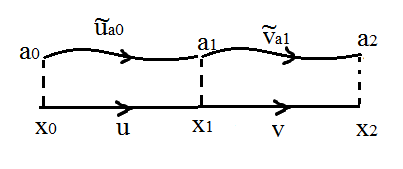
\includegraphics[scale = 0.6]{17-5.png}}
	\end{figure}
	\begin{enumerate}
		\item Покажем: $g$ корректно определено\\
		Из условия (2): существует петля $w: I\rightarrow E$ в $a_0$, такая что $f \circ uv^{-1} = p \circ w$\\
		$(f \circ u)(f \circ v^{-1}) = (f \circ u)(f \circ v)^{-1} \Rightarrow (f \circ u) \underset{p}{\simeq} (p \circ w)(f \circ v) \Rightarrow (f \circ u)_{a_0}^{\sim} \underset{p}{\simeq} w \circ (f \circ v)_{a_0}^{\simeq} \Rightarrow (f \circ u)_{a_0}^{\sim} (1) = (f \circ v)_{a_0}^{\sim} (1) \Rightarrow g$ корректно определенно
		\item Непрерывность $g$\\
		Зафиксируем $\forall y\in Y$. Достаточно доказать: $g$ непрерывно в некоторой окрестности y\\
		Обозначим: $x = f(y)$\\
		Пусть $U\ni x$ -- ровно накрытая окрестность. Существует линейно связная окрестность $V$ точки $y$, такая что $f(V)\subset U$\\
		Существует открытое $W\subset E, такая что {p|}_w$:\ $W\Rightarrow U$ -- гомеоморфизм, и такой что $g(y) \in W$\\
		Обозначим $s = ({p|}_w)^{-1}:\ U \rightarrow W$\\
		Достаточно доказать: ${g|}_v = so({f|}_v) (*)$\\
		Пусть $z\in V, V$ -- линейно связно $\Rightarrow$ выберем $v\in P(y,z), v(I) \subset V$\\
		ПУсть $u\in P(y_0,y) \Rightarrow g(z) = (fouv)_{a_0}^{\sim}$ (1)\\
		Заметим: $(fov)_{a}^{\sim} = sofov$\\
		Обозначим $a = g(y)$ (так как они оба поднимают $fov$ и начинаются в $a$)\\
		$(fouv)_{a_0}^{\sim} = (fou)_{a_0}^{\sim} \cdot (fov)_{a_0}^{\sim} = (fou)_{a_0}^{\sim} \cdot (sofov) \Rightarrow g(z) = (sofov) (1) = (sof)(z) = s(f(z)) \Rightarrow (*)$ -- доказано $\Rightarrow g$ непрерывно что и требовалось доказать
	\end{enumerate}
	\textbf{Следствие}: $p: E\Rightarrow X$ -- накрытие, $x_0 \in X a_0 \in p^{-1} (x_0), Y$ -- односвязно и локально линейно связно\\
	Тогда для любого непрерывного $f: Y \Rightarrow X$, такого что $f(y_0) = x_0$ существует единственное поднятие $g: Y \rightarrow E$ отображения $f$, такое что $g(y_0) = a_0$


\newpage
%-----------------------------------------------------------------------------
	\section{}
	\textbf{Пунктированные накрытия и их морфизмы. Теорема о классификации морфизмов связных пунктированных накрытий и критерий их изоморфизма в терминах подгрупп фундаментальной группы базы}\\
	\\
	\\
	\textbf{Теорема об эквивалентности категории накрытия}: Функтор $\mathcal{F}: \text{Cov}(X) \rightarrow G-Sets$ -- эквивалентность категорий\\
	Фнуктор $\mathscr{G}: G-Sets \rightarrow \text{Cov}(X)$ -- его квазиобр.\\
	\textbf{Следствие 1}: Функтор $\mathcal{F}: \text{Cov}_0 (X) \rightarrow Tr G-Sets$ -- эквивалентность категорий\\
	\textbf{Доказательство}: с учетом основной теоремы достаточно доказать:\\
	$\mathscr{G} (Tr G-Sets) \subset \text{Cov}_0 (X)$\\
	Пусть $S$ -- транзитивно, $G$-множество, $S\cong \mathcal{F} (\mathscr{G} (S)) = p_s^{-1} (x_0)$\\
	Действие монодромии на $p_s^{-1} (x_0)$ транзитивно $\mathscr{G}$ -- связно(было)\\
	\textbf{Следствие 2( теорема о классификации связных накрытий)}\\
	Функтор $\mathcal{F}$ порождает биекцию между множеством классов изоморфизма связных накрытий X и множеством подгрупп в G по правилу:\\
	$(E,p) \rightarrow \text{\text{Stabs}}(\mathcal{F} (E,p))$ = класс сопряженности подгруппы $Im p_{x,a} \subset G$, где $a$ -- любая точка из слоя $p_s^{-1} (x_0)$\\
	\textbf{Обозначение}: Функтор $\mathcal{F}^{*}: \text{Cov}_0^* (X,x_0) \rightarrow Sub(G)$\\
	$\mathcal{F}^{*} ((E,p),a) = Im p_{*,a} \subset G$\\
	Знаем: $\mathscr{G}$ -- строгий и полный\\
	для любой подгруппы $H\subset G обозначим \mathscr{G}^* (H) = (\mathscr{G}(G\diagup H), a_H)$, где $a_H = [(H,e)]\in (G\diagup H) \underset{G}{\times} \underset{\sim}{X}$\\
	Заметим: $p_s (a_H) = x_0$\\
	Пусть $H\subset K \subset G$ -- подгруппа, $i_{H;K}: H \subset K$ -- отображение включения\\
	$q_{H;K}: G\diagup H \rightarrow G\diagup K, Hg \rightarrow Kg$ -- морфизм G-множеств\\
	$\mathscr{G}^* (i_{H;K}) = \mathscr{G}(q_{H;K}):\ \mathscr{G}(G\diagup H) \rightarrow \mathscr{G} (G\diagup K)$; заметим: $\mathscr{G}^* (a_H) = a_k$\\
	Получим функтор $\mathscr{G}^*: Sub(G)\rightarrow \text{Cov}_0^* (X,x_0)$\\
	\textbf{Следствие 3}: $\mathcal{F}^*: \text{Cov}_0^* (X,x_0) \rightarrow Sub(G)$ -- эквивалентность категорий\\
	$\mathscr{G}^*:\ Sub(G) \rightarrow \text{Cov}_0^* (X,x_0)$ -- его квазиобр.\\
	Более того: $\mathcal{F}^* \mathscr{G}^* =  \text{id}_{Sub(G)}$\\
	\textbf{Доказательство}: с учетом Леммы 2(билет 25) достаточно доказать: $\mathcal{F}^* \mathscr{G}^* =  \text{id}_{Sub(G)}$\\
	Пусть $H\subset G$ -- подгруппа\\
	$\mathscr{G} (G\diagup H) \underset{p_{G\diagup H}}{\rightarrow} X$\\
	Обозначим: $p = p_{G\diagup H}$\\
	\textbf{Хотим доказать}: $H = Im(p_{*},a)$, где $a = a_H$\\
	Пусть $v$ -- петля в $x_0$\\
	$[v] \in Im(p_{*},a) \Leftrightarrow \overset{\sim}{v_a}$ -- петля, то есть $\overset{\sim}{v_a} (1) = a$\\
	Из Леммы 1: $\overset{\sim}{v_a} (1) = [(H,[v])] = [(H[v],e)]$\\
	Поэтому: $\overset{\sim}{v_a} (1) \Leftrightarrow [(H[v],e)] = [H,e] \Leftrightarrow$ (так как $S \underset{G}{\times} G \cong S, [(s,e)]\rightarrow s) H[v] = H \Leftrightarrow [v]\in H \Rightarrow Im(p_{*},a) = H$ что и требовалось доказать\\
	\textbf{Следствие 4}(теорема о классификации связных накрытий с отмеченными точками): Функтор $\mathcal{F}^*$ порождает биекцию между множеством классов изоморфизма связных пунктиных накрытий X и множеством подгрупп в $G$ по правилу $((E,p),a) \rightarrow Im(p_{*},a)$\\
	\begin{figure}[h]
		\center{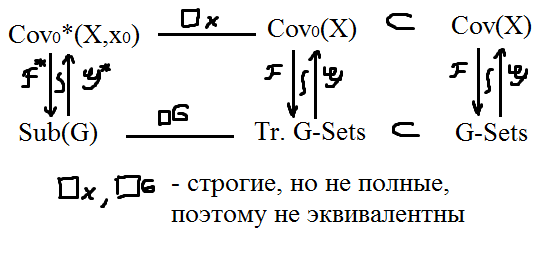
\includegraphics[scale = 0.55]{26-1.png}}
	\end{figure}\\


\newpage
%-----------------------------------------------------------------------------
	\section{}
	\textbf{Действие монодромии. Условие его транзитивности. Описание стабилизатора точки слоя при действии монодромии}\\
	\\
	\textbf{Теорема}: $p: E\rightarrow X$ -- накрытие $x_0 \in X$. Тогда существует правое действие ${\pi}_1 (X, x_0)$ на $p^{-1} (x_0)$, заданное формулой $y \cdot [u] = \overset{\sim}{u_y} (1) (y\in p^{-1} (x_0), [u] \in {\pi}_1 (X, x_0)) (*)$, где $\overset{\sim}{u_y}$ -- поднятие $u$, такое что $\overset{\sim}{u_y} (0) = y$\\
	Если $E$ -- линейно связно, то это действие транзитивно\\
	Если $E$ односвязно, то это действие свободно\\
	\textbf{Определение}: действие $(*)$ называется действием монодромии\\
	\textbf{Доказательство}: $P(\overset{\sim}{u_y} (1)) = u(1) = x_0$ (для любой петли в $x_0$) $\Rightarrow \overset{\sim}{u_y} (1) \in p^{-1} (x_0)$\\
	Из теоремы выше: формула $(*)$ корректно определяет отображение $p^{-1} (x_0) \times {\pi}_1 (X,x_0) \rightarrow p^{-1} (x_0), (y,[u]) = y\times [u] = \overset{\sim}{u_y} (1)$\\
	Покажем: это действие\\
	$\forall y \in p^{-1} (x_0): y\cdot [e] = \overset{\sim}{e_y} (1) = y$, так как $\overset{\sim}{e_y}$ -- постоянная петля в $y$\\
	$\forall y \in p^{-1} (x_0), \forall [u], [v] \in {\pi}_1 (X,x_0)$\\
	\begin{comment}
	\begin{figure}[h]
	\center{\includegraphics[scale = 0.6]{15-2.png}}
	\end{figure}\\
	\end{comment}
	Обозначим: $z = y\cdot [u] = \overset{\sim}{u_y} (1) \Rightarrow (y [u]) \cdot [v] = z \cdot [v] = \overset{\sim}{v_z} (1)\\
	\overset{\sim}{u_y} \cdot \overset{\sim}{v_z}$ -- поднятие $u\cdot v$\\
	$(\overset{\sim}{u_y} \cdot \overset{\sim}{v_z}) (0) = \overset{\sim}{u_y} (0) = y \Rightarrow \overset{\sim}{u_y} \cdot \overset{\sim}{v_y} = \overset{\sim}{(uv)_y}\\
	y\cdot ([u][v]) = y[u\cdot v] = \overset{\sim}{(uv)_y} (1) = (\overset{\sim}{u_y} \cdot \overset{\sim}{v_z}) (1) = \overset{\sim}{v_z} (1) \Rightarrow (y\cdot [u])[v] = y([u][v]) \Rightarrow (*)$ определяет действие\\
	\begin{comment}
	\begin{figure}[h]
	\center{\includegraphics[scale = 0.6]{15-3.png}}
	\end{figure}\\
	\end{comment}
	Пусть $E$ линейно связно, $y,z \in p^{-1} (x_0)$\\
	Выберем $v \in P(y,z)$, обозначим $u = p\cdot v \Rightarrow u$ -- петля в $x_0, v = \overset{\sim}{u_y} \Rightarrow y\cdot [u] = v(1) = z \Rightarrow$ действие транзитивно\\
	Пусть $E$ односвязно, $y\in p^{-1} (x_0), [u]\in {\pi}_1 (X,x_0), y[u] = y$, то есть $y = \overset{\sim}{u_y} (1) \Rightarrow \overset{\sim}{u_y}$ -- петля в $y \Rightarrow \overset{\sim}{u_y} \simeq e_y \Rightarrow u \underset{p}{\simeq} e_{x_0}$, то есть $[u] = [e_{x_0}] \Rightarrow$ действие свободно что и требовалось доказать\\
	Следствие: $p: E\rightarrow X$ -- накрытие, $E$ -- односвязно $\Rightarrow \forall x_0 \in X, \forall y\in p^{-1} (x_0)$, отображение ${\pi}_1 (x,x_0) \rightarrow p^{-1} (x_0), [u] \rightarrow y[u]$ -- биекция\\



\newpage
%-----------------------------------------------------------------------------
	\section{}
	\textbf{Морфизмы G-множеств. Изоморфизм между орбитой и множеством смежных классов по стабилизатору. Следствие: изоморфизм между слоем накрытия и множеством смежных классов фундаментальной группы базы накрытия по образу фундаментальной группы накрывающего пространства.}\\
	\\	
	\textbf{Определение}: $X, Y$ -- правые $G$-множества\\
	Отображение $\phi:\ X\rightarrow Y$ -- морфизм $G$-множеств ($G$-эквивалентное отображение) $\Leftrightarrow \phi (x\cdot g) = \phi (x) \cdot g (x\in X, g\in G$)\\
	Правые $G$-множества и их морфизм образуют категорию. Обозначают ее $G-Sets$\\
	\textbf{Предложение}: $X$ -- правое $G$-множество, $x\in X, x\in X$. Существует изоморфизм правых $G$-множеств\\
	$\phi:\ {G\diagup}_{\text{Stab}(X)} \overset{\sim}{\rightarrow} x\cdot G, \phi(\text{Stab}(x)\cdot g) = x\cdot g (g\in G)$.\\
	В частности, если $X$ транзитивно, то $\phi$-изоморфизм ${G\diagup}_{\text{Stab}(X)}$ на $X$.\\
	\textbf{Доказательство}: пусть $g, h \in G$\\
	$\text{Stab}(x)\cdot g = \text{Stab}(x)\cdot h \Leftrightarrow g\cdot h^{-1} \in \text{Stab}(x) \Leftrightarrow x\cdot g\cdot x^{-1} = x\Leftrightarrow x\cdot g = x\cdot h$\\
	Поэтому $\phi$ -- корректно определенно и инъективно. Очевидно, $\phi$ -- сюръективно и является морфизмом G-множеств что и требовалось доказать\\
	Гомоморфизм фундаментальных групп, индуцированный накрывающих отображением.\\
	$p: E\rightarrow X -- накрытие, x_0 \in X, a\in p^{-1} (x_0)\\
	p_x: {\pi}_1 (E, a) \rightarrow {\pi}_1 (X, x_0)$\\
	Напоминания: Пусть $x_1\in X, u\in P(x_0,x_1), \overset{\sim}{u_a}$ -- поднятие $u$, такое что $\overset{\sim}{u_a} (0) = a$ (оно существует и единственное)\\
	Если $v,u\in P(x_0,x_1)$, то $u \underset{p}{\simeq} v \Leftrightarrow \overset{\sim}{u_a} \underset{p}{\simeq} \overset{\sim}{v_a} \Rightarrow \overset{\sim}{u_a} (1) = \overset{\sim}{v_a} (1)$\\
	\begin{figure}[h]
		\center{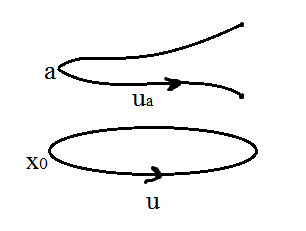
\includegraphics[scale = 0.6]{16-1.png}}
	\end{figure}\\
	Действие монодромии: $p^{-1} (x_0) \times {\pi}_1 (X, x_0) \rightarrow p^{-1} (x_0), (a,[u])\rightarrow a[u] = \overset{\sim}{u_a} (1)$\\
	\textbf{Теорема}: $p: E\rightarrow X$ -- накрытие, $x_0 \in X, a\in p^{-1} (x_0)$
	\begin{enumerate}
		\item $p_{\ast}:\ {\pi}_1 (E,a) \rightarrow {\pi}_1 (X,x_0)$ -- мономорфизм
		\item $Im p_{\ast} = \{ [u]:\ \overset{\sim}{u_a}$ -- петля$\}$
		\item $Im p_{\ast} = \text{Stab}(a)$ при действии монодромии
		\begin{figure}[h]
			\center{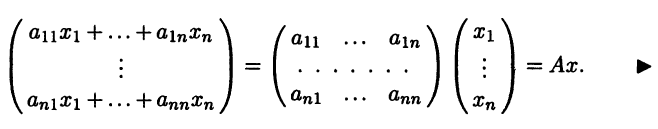
\includegraphics[scale = 0.6]{16-2.png}}
		\end{figure}
	\end{enumerate}
	\textbf{Доказательство}:
	\begin{enumerate}
		\item Пусть $[v] \in Ker p_{\ast}$. Обозначим $u = p\cdot v$\\
		$u \underset{p}{\simeq} e_{x_0} \Rightarrow \overset{\sim}{u_a} \underset{p}{\simeq} {(\overset{\sim}{e_{x_0}})}_a ( = e_a), то есть [v] = [e_a] \in {pi}_1 (E,a)$
		\item $[u]\in Im p_{\ast} \Leftrightarrow u \underset{p}{\simeq} p \circ v$ для некоторой петли $v$ в $a \Leftrightarrow \overset{\sim}{u_a} \underset{p}{\simeq} v$ для некоторой петли $v$ в $a \Leftrightarrow \overset{\sim}{u_a}$ -- петля
		\item $\overset{\sim}{u_a} -петля \Leftrightarrow \overset{\sim}{u_a} (1) = a \Leftrightarrow a = a\cdot [u] \Leftrightarrow [u] \in St(a)$ что и требовалось доказать
	\end{enumerate}
	\textbf{Следствие}: $p: E\rightarrow X$ -- накрытие\\
	$E$ -- линейно связно, $x_0 \in X, a\in p^{-1} (x_0)$. Существует изоморфизм правых ${\pi}_1 (X,x_0)$ -- множеств\\
	${{\pi}_1 (X,x_0) \diagup}_{Im p_{\ast}} \overset{\sim}{\rightarrow} p^{-1} (x_0), (Im p_{\ast})\cdot [u] \rightarrow a\cdot [u] = \overset{\sim}{u_a} (1)$\\
	\textbf{Доказательство}: из п.(3) теоремы и транзитивности монодромии что и требовалось доказать


\newpage
%-----------------------------------------------------------------------------
	\section{}
	\textbf{Морфизмы накрытий. Ограничение морфизма накрытий на слой является морфизмом $\pi_1(X, x_0)$ -- множеств. Морфизмы транзитивных G-множеств с отмеченной точкой: единственность и критерий существования. Теорема о классификации морфизмов связных накрытий (биективность соответствия между морфизмами накрытий и морфизмами соответствующих $\pi_1(X, x_0)$ -- множеств).}\\
	\\	
	\\
	Предл: $G$ -- группа, $X, Y$ -- прав. $G$ мн-ва; $x \in X, y \in Y$\\
	\begin{enumerate}
		\item $\forall$ морфизм $\varphi: X \rightarrow Y$\\
		$\text{Stab}(x) \subset \text{Stab}(\varphi(x))$
		\item $X$ -- транзитивно $\Rightarrow \exists$ не более одного морфизма $\varphi: X \rightarrow Y$, т.ч $\varphi(x) = y$
		\item Если $X$ -- транзитивно, то такой $\varphi$ существует $\Leftrightarrow\ \text{Stab}(x) \subset \text{Stab}(y)$
	\end{enumerate}
	\textbf{Доказательство}:\\ 
	(1) $\forall g \in \text{Stab}(x)\\
	\varphi(x)g = \varphi(xg) = \varphi(x) \Rightarrow g \in \text{Stab}(\varphi(x))$\\
	(2) Если $\varphi(x) = g$, то $\varphi(xg) = yg$, $\forall g \in G$\\
	(3) $(\Rightarrow)$: из (1)\\
	$(\Leftarrow)$: Определим $\varphi: X \rightarrow Y$ так $\varphi(xg) = yg$, $\forall g \in G$\\
	Пусть $xg_1 = xg_2 \Rightarrow xg_1g_2^{-1} = x \Rightarrow g_1g_2^{-1} \in \text{Stab}(x) \subset \text{Stab}(y) \Rightarrow yg_1 = yg_2 \Rightarrow \varphi$ корректно определено\\
	Очев, $\varphi$ -- морфизм $G$-множеств, $\varphi(x) = y$, что и требовалось доказать\\
	Обозн: $X$ -- транзитивное $G$-мн-во,\\
	$\text{\text{Stabs}}(X) = \text{Stab}(x)|x \in X$\\
	\textbf{Наблюдение}: для $\forall x, \forall g \in G$\\
	$\text{Stab}(xg) = g^{-1}\text{Stab}(x)g$\\
	$X$ -- транз, $\Rightarrow\ \text{Stab}(X) = \{g^{-1}\text{Stab}(x)g|g \in G\}$(*) -- множество всех подгрупп, сопряженных $\text{Stab}(x)$\\
	Предл. следующие утверждения эквивалентны:\\
	\begin{enumerate}
		\item $X \simeq Y$
		\item $\text{\text{Stabs}}(X) = \text{\text{Stabs}}(Y)$
	\end{enumerate}
	\textbf{Доказательство}: $(1) \Rightarrow (2)$\\
	$\text{Stab}(x) = \text{Stab}\varphi(x) \Rightarrow$ по $(*) \text{\text{Stabs}}(X) = \text{\text{Stabs}}(Y)$\\
	$(2) \Rightarrow (1)$\\
	Зафиксируем $\forall x \in X, \exists y \in Y$, т.ч $\text{Stab}(x) = \text{Stab}(y)$\\
	$\exists$ морфизм $\varphi: X \rightarrow Y$ и $\phi: Y \rightarrow X$, такие что $\varphi(x) = y$ и $\phi(y) = x\ \Rightarrow\ (\phi \varphi)(x) = x\ \Rightarrow\ \phi \varphi =  \text{id}_x\ \Rightarrow\ \varphi$ -- изоморфизм, что и требовалось доказать\\
	Th: Функтор $\mathcal{F}: \ \text{Cov}(X)\rightarrow {\pi}_1 (X, x_0)$ строгий и полный\\
	\textbf{Доказательство}: (строгость)\\
	Пусть $f, g: (E,p) \rightarrow (F,q)$ -- морфизм в $\text{Cov}(X)$, $f|_{p^{-1}(x_0)} = g|_{p^{-1}(x_0)}$\\
	$\{E_{i}|i \in I\}$ -- связные компоненты $E, p_i = p|_{E_i}: E_i \rightarrow X$\\
	$\forall i \in I: \ f|_{p^{-1}(x_0)} = g|_{p^{-1}(x_0)}$\\
	$f,g|_{E_i}: (E_i,p_i) \rightarrow (F,q)$, $E_i$ -- связно $\Rightarrow\ f|_{E_i} = g|_{E_i}\ \forall i\ \Rightarrow\ f = g\ \Rightarrow\ \mathcal{F}$ строгий\\
	(полнота) Пусть $G = {\pi}_1 (X, x_0);$ пусть $\varphi: p^{-1}(x_0) \rightarrow q^{-1}(x_0)$\\
	Обозначим $\varphi_i: \varphi|{p_i}^{-1}(x_0): {p_i}^{-1}(x_0) \rightarrow q^{-1}(x_0)$\\
	Зафиксируем $\forall a \in {p_i}^{-1}(x_0),\ b = \varphi_i(a);\ \text{Stab}(a) \subset \text{Stab}(b)\ \Rightarrow\ \exists!$ морфизм накрытий $f_i: (E_i,p_i) \rightarrow (F,q)$, т.ч $f_i(a) = b$\\
	$\varphi_i: p^{-1}(x_0) \rightarrow q^{-1}(x_0)$ переводит $a$ в $b\ \Rightarrow\ f_i|{p_i}^{-1}(x_0) = \varphi_i$\\
	Определим $f: E \rightarrow F$ так $f|_{E_i} = f_i$\\
	Очевидно $f$ -- морфизм накрытий и $f|{p}^{-1}(x_0) = \varphi\ \Rightarrow\ \mathcal{F}$ полный\\
	Как следствие $\mathcal{F}: \text{Cov}(X) \rightarrow Tr{\pi}_1 (X, x_0)$ строгий и полный\\


\newpage
%-----------------------------------------------------------------------------
	\section{}
	\textbf{Действие группы сопряжениями (на себе и на множестве подгрупп). Сопряженность стабилизаторов точек из одной орбиты. Критерий изоморфизма транзитивных G-множеств. Критерий изоморфизма накрытий в терминах подгрупп фундаментальной группы базы}\\
	\\
	Изоморфизмы транзитивных $G$-множеств и классы сопряженных подгрупп. Функтор $\mathcal{F}$ из категории накрытия $\text{Cov}(X)$ в категорию ${\pi}_1 (X, x_0)$-множеств. Его строгость и полнота. Следствие: критерий изоморфизма связных накрытий в $\text{Cov}(X)$}\\
	\\
	Предл: $G$ -- группа, $X, Y$ -- прав. $G$ мн-ва; $x \in X, y \in Y$\\
	\begin{enumerate}
	\item $\forall$ морфизм $\varphi: X \rightarrow Y$\\
	$\text{Stab}(x) \subset \text{Stab}(\varphi(x))$
	\item $X$ -- транзитивно $\Rightarrow \exists$ не более одного морфизма $\varphi: X \rightarrow Y$, т.ч $\varphi(x) = y$
	\item Если $X$ -- транзитивно, то такой $\varphi$ существует $\Leftrightarrow\ \text{Stab}(x) \subset \text{Stab}(y)$
	\end{enumerate}
	\textbf{Доказательство}:\\ 
	(1) $\forall g \in \text{Stab}(x)\\
	\varphi(x)g = \varphi(xg) = \varphi(x) \Rightarrow g \in \text{Stab}(\varphi(x))$\\
	(2) Если $\varphi(x) = g$, то $\varphi(xg) = yg$, $\forall g \in G$\\
	(3) $(\Rightarrow)$: из (1)\\
	$(\Leftarrow)$: Определим $\varphi: X \rightarrow Y$ так $\varphi(xg) = yg$, $\forall g \in G$\\
	Пусть $xg_1 = xg_2 \Rightarrow xg_1g_2^{-1} = x \Rightarrow g_1g_2^{-1} \in \text{Stab}(x) \subset \text{Stab}(y) \Rightarrow yg_1 = yg_2 \Rightarrow \varphi$ корректно определено\\
	Очев, $\varphi$ -- морфизм $G$-множеств, $\varphi(x) = y$, что и требовалось доказать\\
	Обозн: $X$ -- транзитивное $G$-мн-во,\\
	$\text{\text{Stabs}}(X) = \text{Stab}(x)|x \in X$\\
	\textbf{Наблюдение}: для $\forall x, \forall g \in G$\\
	$\text{Stab}(xg) = g^{-1}\text{Stab}(x)g$\\
	$X$ -- транз, $\Rightarrow\ \text{Stab}(X) = \{g^{-1}\text{Stab}(x)g|g \in G\}$(*) -- множество всех подгрупп, сопряженных $\text{Stab}(x)$\\
	Предл. следующие утверждения эквивалентны:\\
	\begin{enumerate}
	\item $X \simeq Y$
	\item $\text{\text{Stabs}}(X) = \text{\text{Stabs}}(Y)$
	\end{enumerate}
	\textbf{Доказательство}: $(1) \Rightarrow (2)$\\
	$\text{Stab}(x) = \text{Stab}\varphi(x) \Rightarrow$ по $(*) \text{\text{Stabs}}(X) = \text{\text{Stabs}}(Y)$\\
	$(2) \Rightarrow (1)$\\
	Зафиксируем $\forall x \in X, \exists y \in Y$, т.ч $\text{Stab}(x) = \text{Stab}(y)$\\
	$\exists$ морфизм $\varphi: X \rightarrow Y$ и $\phi: Y \rightarrow X$, такие что $\varphi(x) = y$ и $\phi(y) = x\ \Rightarrow\ (\phi \varphi)(x) = x\ \Rightarrow\ \phi \varphi =  \text{id}_x\ \Rightarrow\ \varphi$ -- изоморфизм, что и требовалось доказать\\
	Th: Функтор $\mathcal{F}: \ \text{Cov}(X)\rightarrow {\pi}_1 (X, x_0)$ строгий и полный\\
	\textbf{Доказательство}: (строгость)\\
	Пусть $f, g: (E,p) \rightarrow (F,q)$ -- морфизм в $\text{Cov}(X)$, $f|_{p^{-1}(x_0)} = g|_{p^{-1}(x_0)}$\\
	$\{E_{i}|i \in I\}$ -- связные компоненты $E, p_i = p|_{E_i}: E_i \rightarrow X$\\
	$\forall i \in I: \ f|_{p^{-1}(x_0)} = g|_{p^{-1}(x_0)}$\\
	$f,g|_{E_i}: (E_i,p_i) \rightarrow (F,q)$, $E_i$ -- связно $\Rightarrow\ f|_{E_i} = g|_{E_i}\ \forall i\ \Rightarrow\ f = g\ \Rightarrow\ \mathcal{F}$ строгий\\
	(полнота) Пусть $G = {\pi}_1 (X, x_0);$ пусть $\varphi: p^{-1}(x_0) \rightarrow q^{-1}(x_0)$\\
	Обозначим $\varphi_i: \varphi|{p_i}^{-1}(x_0): {p_i}^{-1}(x_0) \rightarrow q^{-1}(x_0)$\\
	Зафиксируем $\forall a \in {p_i}^{-1}(x_0),\ b = \varphi_i(a);\ \text{Stab}(a) \subset \text{Stab}(b)\ \Rightarrow\ \exists!$ морфизм накрытий $f_i: (E_i,p_i) \rightarrow (F,q)$, т.ч $f_i(a) = b$\\
	$\varphi_i: p^{-1}(x_0) \rightarrow q^{-1}(x_0)$ переводит $a$ в $b\ \Rightarrow\ f_i|{p_i}^{-1}(x_0) = \varphi_i$\\
	Определим $f: E \rightarrow F$ так $f|_{E_i} = f_i$\\
	Очевидно $f$ -- морфизм накрытий и $f|{p}^{-1}(x_0) = \varphi\ \Rightarrow\ \mathcal{F}$ полный\\
	Как следствие $\mathcal{F}: \text{Cov}(X) \rightarrow Tr{\pi}_1 (X, x_0)$ строгий и полный\\
	Критерий изоморфизма накрытий в $\text{Cov}(X)$:\\
	$(E,p)\sim (F,q)$ -- накрытия $X$; $E,F$ -- связны, $x_0 \in X, a \in p^{-1}(x_0), b \in q^{-1}(x_0)$\\
	$((E, p), a_0) \simeq ((F,q), b_0)$ в $\text{Cov}_0^{*}(X, x_0)\ \Leftrightarrow\ Im p_{*,a}$ и $Im q_{*,b}$ сопряжены в ${\pi}_1(X, x_0)$\\
	\textbf{Доказательство}: из того, что $\mathcal{F}^{*}$ и $\mathcal{F}$ строгие и полные и из леммы, что и требовалось доказать\\
	


\newpage
%-----------------------------------------------------------------------------
	\section{}
	\textbf{Нормализатор подгруппы в группе. Описание группы автоморфизмов транзитивного Gмножества в терминах группы G. Описание группы автоморфизмов связного накрытия в терминах фундаментальной группы базы. Следствие: группа автоморфизмов односвязного накрытия.}\\
	\\	



\newpage
%-----------------------------------------------------------------------------
	\section{}
	\textbf{Универсальное накрытие и его универсальное свойство. Относительно односвязные подмножества и полулокально односвязные пространства. Примеры и контрпримеры. Необходимое условие существования универсального накрытия.}\\
	\\	
	\textbf{Определение}: Накрытие: $p: \overset{\sim}{X} \rightarrow X$ называется универсальным $\Leftrightarrow \overset{\sim}{X}$ односвязно.\\
	Предл: Пусть $p: \overset{\sim}{X} \rightarrow X$ -- универсальное накрытие, $x_0 \in X, a\in p^{-1}(x_0)$. Тогда $((\overset{\sim}{X}, a), p)$ -- инициальный объект в $\text{Cov}_{0}^{*}(X,x_0)$\\
	Пусть $q: F\rightarrow X$ -- накрытие, А -- связно, $b\in q^{-1}(x_0) \subset F$\\
	Знаем: $\exists$ не более одного морфизма.\\
	$(\overset{\sim}{X}, p) \rightarrow (F,p)$ в $\text{Cov}_{0}^{*}(X,x_0)$ и он $\exists \Leftrightarrow Im p_{*,a} \subset Im q_{*,a}$ Последнее услвоие выполнено, т.к. $\overset{\sim}{X}$ односвязно и $Im p_{*,a} = {e}$\\
	\textbf{Предл}: След свойства подмножества $U\subset X$ эквивалентны\\
	\begin{enumerate}
		\item $\forall x \in U$ гомоморфизм $i_{*}: (U,x)\rightarrow \pi_1(X,x)$ индуциров. включением $i: U\rightarrow X$ тривиален. (то есть $Im i_x = {e}$)
		\item $\forall$ петля в U гомотопна в Х постоянной петле
		\item $\forall x_0, x \in U$ Любые пути $u,v: I\rightarrow U$ из $x_0$ в х, гомотопны в Х
	\end{enumerate}
	\textbf{Доказательство}:\\
	(1) $\Leftrightarrow$ (2) из определения $i_{*}$\\
	(2) $\Leftrightarrow$ (3) Как для U = X (cм ранее)\\
	\textbf{Определение}: Мн-во $U \subset X$, удовл. условиям (выше) называется относительно односвязным.
	Набл 1: $U \subset X$, отн. односвязно $\Rightarrow$ каждый $v \subset U $ относ. односвязно в X.\\
	\textbf{Определение}: Х наз\\
	\begin{enumerate}
		\item Локально односвязным $\Leftrightarrow \forall x\in X \forall U\ni x \exists$ односвязная окрестность $V\ni x$, т.ч. $V\subset U$
		\item Полулокально односвязным $\Leftrightarrow \forall x\in X \exists$ относительно односвяз. окрестность $U\ni x$
	\end{enumerate}
	Набл 2:\\
	(1) лок. односвязное $\Rightarrow$ полулок. односвяз. и лок линейно связно.\\
	(2) Х -- полулок односвяз. $\Leftrightarrow \forall x \in X\ \forall U\ni x\ \exists$ относ. односвяз. окрестность $V\ni x, V\subset U$\\
	Если вдобавок Х лок лин связно, то $\exists$ линейно связное V с этими свойствами (следует из набл 1)\\
	Предл: Пусть $\exists$ унив. накрытие $p: \overset{\sim}{X} \rightarrow X \Rightarrow$ X -полулок односвязно.\\
	Пусть $x\in X, U\ni x$ ровно накр. окр-ть $\forall$ петля г в U поднимается до $\overset{\sim}{u}$ в $\overset{\sim}{X}$, $\overset{\sim}{X}$ односвязно $\Rightarrow\ \overset{\sim}{u}$ гомотопно в $\overset{\sim}{X}$ пост. петле $\Rightarrow$ г гомотопно в Х пост петле $\Rightarrow$ U относ. односвязно


\newpage
%-----------------------------------------------------------------------------
	\section{}
	\textbf{Теорема о существовании универсального накрытия. Примеры универсальных накрытий.}\\
	\\	
	X -- связное, локально линейно связное, полулокально односвязное топологическоепространство. Тогда $\exists$ универсальное накрытие p: $\overset{\sim}{X} \rightarrow$ X.\\
	Набл. (где искать $\overset{\sim}{X}$?)\\
	Предположим универсальное накрытие p: $\overset{\sim}{X} \rightarrow$ X существует\\
	$\forall x_0,x_1 \in X П(x_0,x_1) = {P(x_0,x_1) \diagup}_{\underset{p}{\simeq}}$\\
	Зафиксируем $x_0 \in X$; пусть $a \in p^{-1}(x_0)$; u,v $\in P(x_0,x), x \in Х$\\
	Знаем: $u \simeq v \Leftrightarrow \overset{\sim}{u_{a}} \simeq \overset{\sim}{v_{a}} \Leftrightarrow \overset{\sim}{u_{a}}(1) = \overset{\sim}{v_{a}}(1)$ (влево из односвязноти $\overset{\sim}{X}$, вправо верно всегда)\\
	Поэтому отобр\\
	$\phi: \underset{x\in X}{\sqcup}$\\
	\begin{figure}[h]
		\center{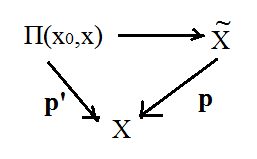
\includegraphics[scale = 0.6]{23-1.png}}
	\end{figure}\\
	$p^{-1}([u]) = u(1)$, диаграмма комутативна\\
	Лемма (Об Атласе) Х -- множество, $X = \underset{i\in I}{\cup} U_i$. Пусть $\forall i\in I$ дано топ пр-во $X_i$ и биекция $\phi_i: U_i \rightarrow X_i$. Предположим, что $\forall i, j \in I$ выполнены условия:\\
	\begin{enumerate}
		\item $\phi_i(U_i \cap U_j)$ -- открыто в $X_i$
		\item "Отображение склейки" $\phi_j \cdot \phi_{i}^{-1}: \phi_i (U_i \cap U_j) \rightarrow \phi_j(U_i \cap U_j) $ непрерывно.	
	\end{enumerate}
	Тогда на X $\exists$ ! топология, в которой все $U_i$ открыт., и в т.ч. все $\phi_i$ -- гомеоморфизмы\\
	\textbf{Терминология}: $(U_I, \phi_i)$ -- карта, $\{(U_i, \phi_i) | i\in I \}$ -- атлас.\\
	\textbf{Идея доказательсва}: Иском топ на Х -- финальная топ порожденная $\{\phi_{i}^{-1} | i\in I \}$ т.е. $u \subset X$ открыто $\Leftrightarrow \phi_i(u \cap U_i)$ открыто в $X_i \forall i$\slash \\
	\textbf{Доказательство}: Зафиксируем $x_0 \in X$ Обозначим $\overset{\sim}{X} = \underset{i\in I}{\sqcup}П(x_0, x) $\\
	$p: \overset{\sim}{X} \rightarrow X, \overset{\sim}{p}([u]) = u(1)$ Обозначим $\forall U \subset X\ \forall x,y \in U П_U(x,y) ( = \{[u] \slash  u\in P(x,y), u(I) \in U\} \subset П(x,y))$\\
	$V = \{U \subset X\ |\ U$ Открыто, лин. связно, относ односвяз$\}$ V покрыв X.\\
	Заметим $\forall U\in V\ \forall x,y \in U П_U(x,y)$ состоит из одного элмента $W_xy\\
	\forall U \in V\ \forall x\in U$ рассмотрим отображения $p^{-1}(U) \underset{\phi_{u,x}}{\overset{\gamma_{u,x}}{\Leftrightarrow}}$ (тут должны быть стелки тудым сюдым сверху фи, снизу вилы дьявола) $П(x_0, x) \times U$\\
	$\gamma_{u,x}(v,y) = vw_{xy} \in p^{-1}(y) \in p^{-1}(U)\\
	\phi_{u,x}(u) = (uw_{yx} , y)$, где $y = u(1)$. Заметим:\\
	$w_{xy} \cdot w_{yz} = w_{xz}\\
	w_{xy} = w^{-1}_{yx}$ Получили что $\phi \gamma$ биекции обратные друг другу.\\
	$(v,y) \rightarrow v\cdot w_{xy} \rightarrow (v\cdot w_{xy} \cdot w_{yx}, y) = (v,y)\\
	u \rightarrow (u\cdot w_{xy}, y) \rightarrow u\cdot w_{xy}\cdot w_{yx} = u$\\
	Снабдим $П(x_0, x)$ дискретной топологией, $П(x_0, x) \times U$ -- топологией произведения. Покажем: сем-во $\{\phi_{u,x}: U\in V, x\in U \}$ удовлет. усл. леммы\\
	Пусть $U,W \in V, x\in U, y\in W$\\
	$\phi_{u,x}(p^{-1}(U) \cap p^{-1}(W) ) = \phi_{u,x}(p^{-1}(U \cap W)) = П(x_0, x)\times (U \cap W)$ -- открыто в $П(x_0, x)\times U \Rightarrow$ усл(1) из леммы выполнено. Проверим (2)\\ 
	Нужно, чтобы $\phi_{v,y} \cdot \gamma_{u,x}: П(x_0, x)\times (U \cap W) \rightarrow П(x_0, y) \times (U \cap W)$ было непрерывным. Зафикс $\forall z\in U \cap W$\\
	Пусть Q -- линейно связн окр-сть z, $Q \subset U \cap W, w_{xt} \in П_W(z,t)$ -- единств. элемен. $\forall t \in Q\ \forall v\in П(x_0, x)$\\
	$(\phi_{v,y} \cdot\ \gamma_{u.x})(v,t) = \phi_{v,y}(v\cdot w_{xt}) = (v\cdot w_{xt} w_{ty}; t) = (v\cdot w_{xz} w_{zt} w_{tz} w_{zy}, t) = (v w_{xz} w_{zy}, t)$ -- непр. отображение. $\Rightarrow$ выполнены условия Леммы $\Rightarrow$ на $\overset{\sim}{X}\ \exists$! топ, в которой все $p^{-1}(U)$ открыты и все $\phi_{u,x}(U\in V, x\in X)$ -- гомеоморфизмы. ИМеем диаграмму.\\
	\begin{figure}[h]
		\center{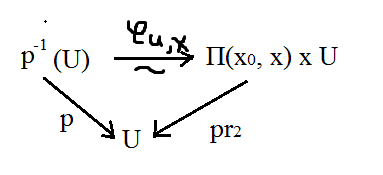
\includegraphics[scale = 0.5]{23-2.png}}
	\end{figure}\\
	$\Rightarrow$ U ровно накрыта p $\Rightarrow p: \overset{\sim}{X} \rightarrow X$ -- накрытие.



\newpage
%-----------------------------------------------------------------------------
	\section{}
	\textbf{Факторизация накрывающего пространства по действию группы. Построение накрытия по подгруппе фундаментальной группы. Теорема о классификации накрытий (с отмеченной точкой и без).}\\
	\\	
